\chapter{Méthodologie} \label{Methodologie}

L'objectif principal du stage est de proposer un outil et une architecture logicielle permettant d'automatiser les \textbf{traitements} nécessaires pour cartographier le risque dans le contexte du paludisme (environnement-santé). Calculer le risque ou les indicateurs revient à définir des chaînes de traitements. Celles-ci sont conceptualisées à partir de l'expertise du domaine.\\


Une première partie d'analyse est dédiée à la compréhension du phénomène (paludisme) et à la conceptualisation des chaînes de traitements. Un modèle conceptuel UML des éléments nécessaires à l'élaboration des indicateurs permet de dégager les facteurs de risque les plus pertinents. A partir des données disponibles, un deuxième modèle UML simplifié servira comme base pour la définition des traitements nécessaires à l'élaboration et au développement de la chaîne. Dans un second temps, des \textbf{modèles conceptuels} des traitements permettent de d'analyser et de définir les différentes étapes nécessaires pour le développement informatique.\\ 

Dans une deuxième partie nous présentons l'architecture informatique des outils ainsi que tout le travail de conception mené autour du développement informatique.\\

Finalement, nous présentons l'opérationnalisation et l'implémentation des deux outils.


\section{Analyse}

Le cycle du paludisme (\ref{cyclemalaria}) permet de comprendre de façon simplifié le développement du paludisme. Ce qui est le plus important à retenir est que le moustique (qui a son propre cycle de développement) pique et infecte l'homme et les parasites se développent dans le foie et le sang de l'homme. Par la suite, un homme porteur du parasite piqué par un moustique sain, infecte celui-ci. Le cycle est donc complexe.


\begin{center}
\begin{figure}[h] \centering
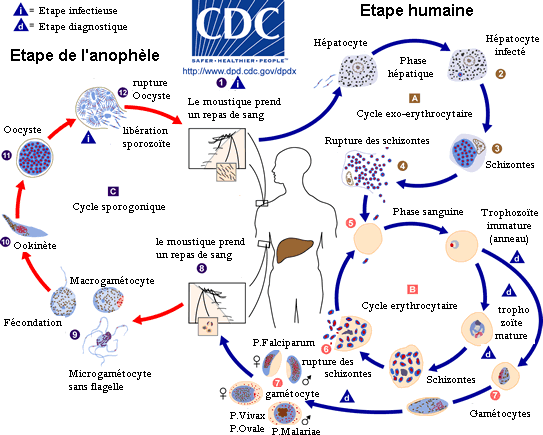
\includegraphics[width=14cm]{malaria}\\
\caption{\label{cyclemalaria} Cycle du paludisme (Extrait de  http://fr.wikipedia.org/wiki/Fichier:Malaria\_LifeCycle)}
\end{figure}
\end{center}

\newpage

\paragraph{Modèle conceptuel des éléments nécessaires à l'élaboration des indicateurs\\\\}
Le modèle conceptuel des éléments nécessaires à l'élaboration des indicateurs (\ref{UML_malaria}) permet d'avoir une vue d'ensemble des facteurs qui interviennent dans le développement du paludisme et qui peuvent être une source de risque. Les grandes caractéristiques du paludisme ont été définies dans une démarche participative lors d'une réunion avec des experts de différents domaines. A partir de ces caractéristiques j'ai élaboré un modèle conceptuel UML.\\

\newpage

\begin{landscape}
\begin{figure}[h]
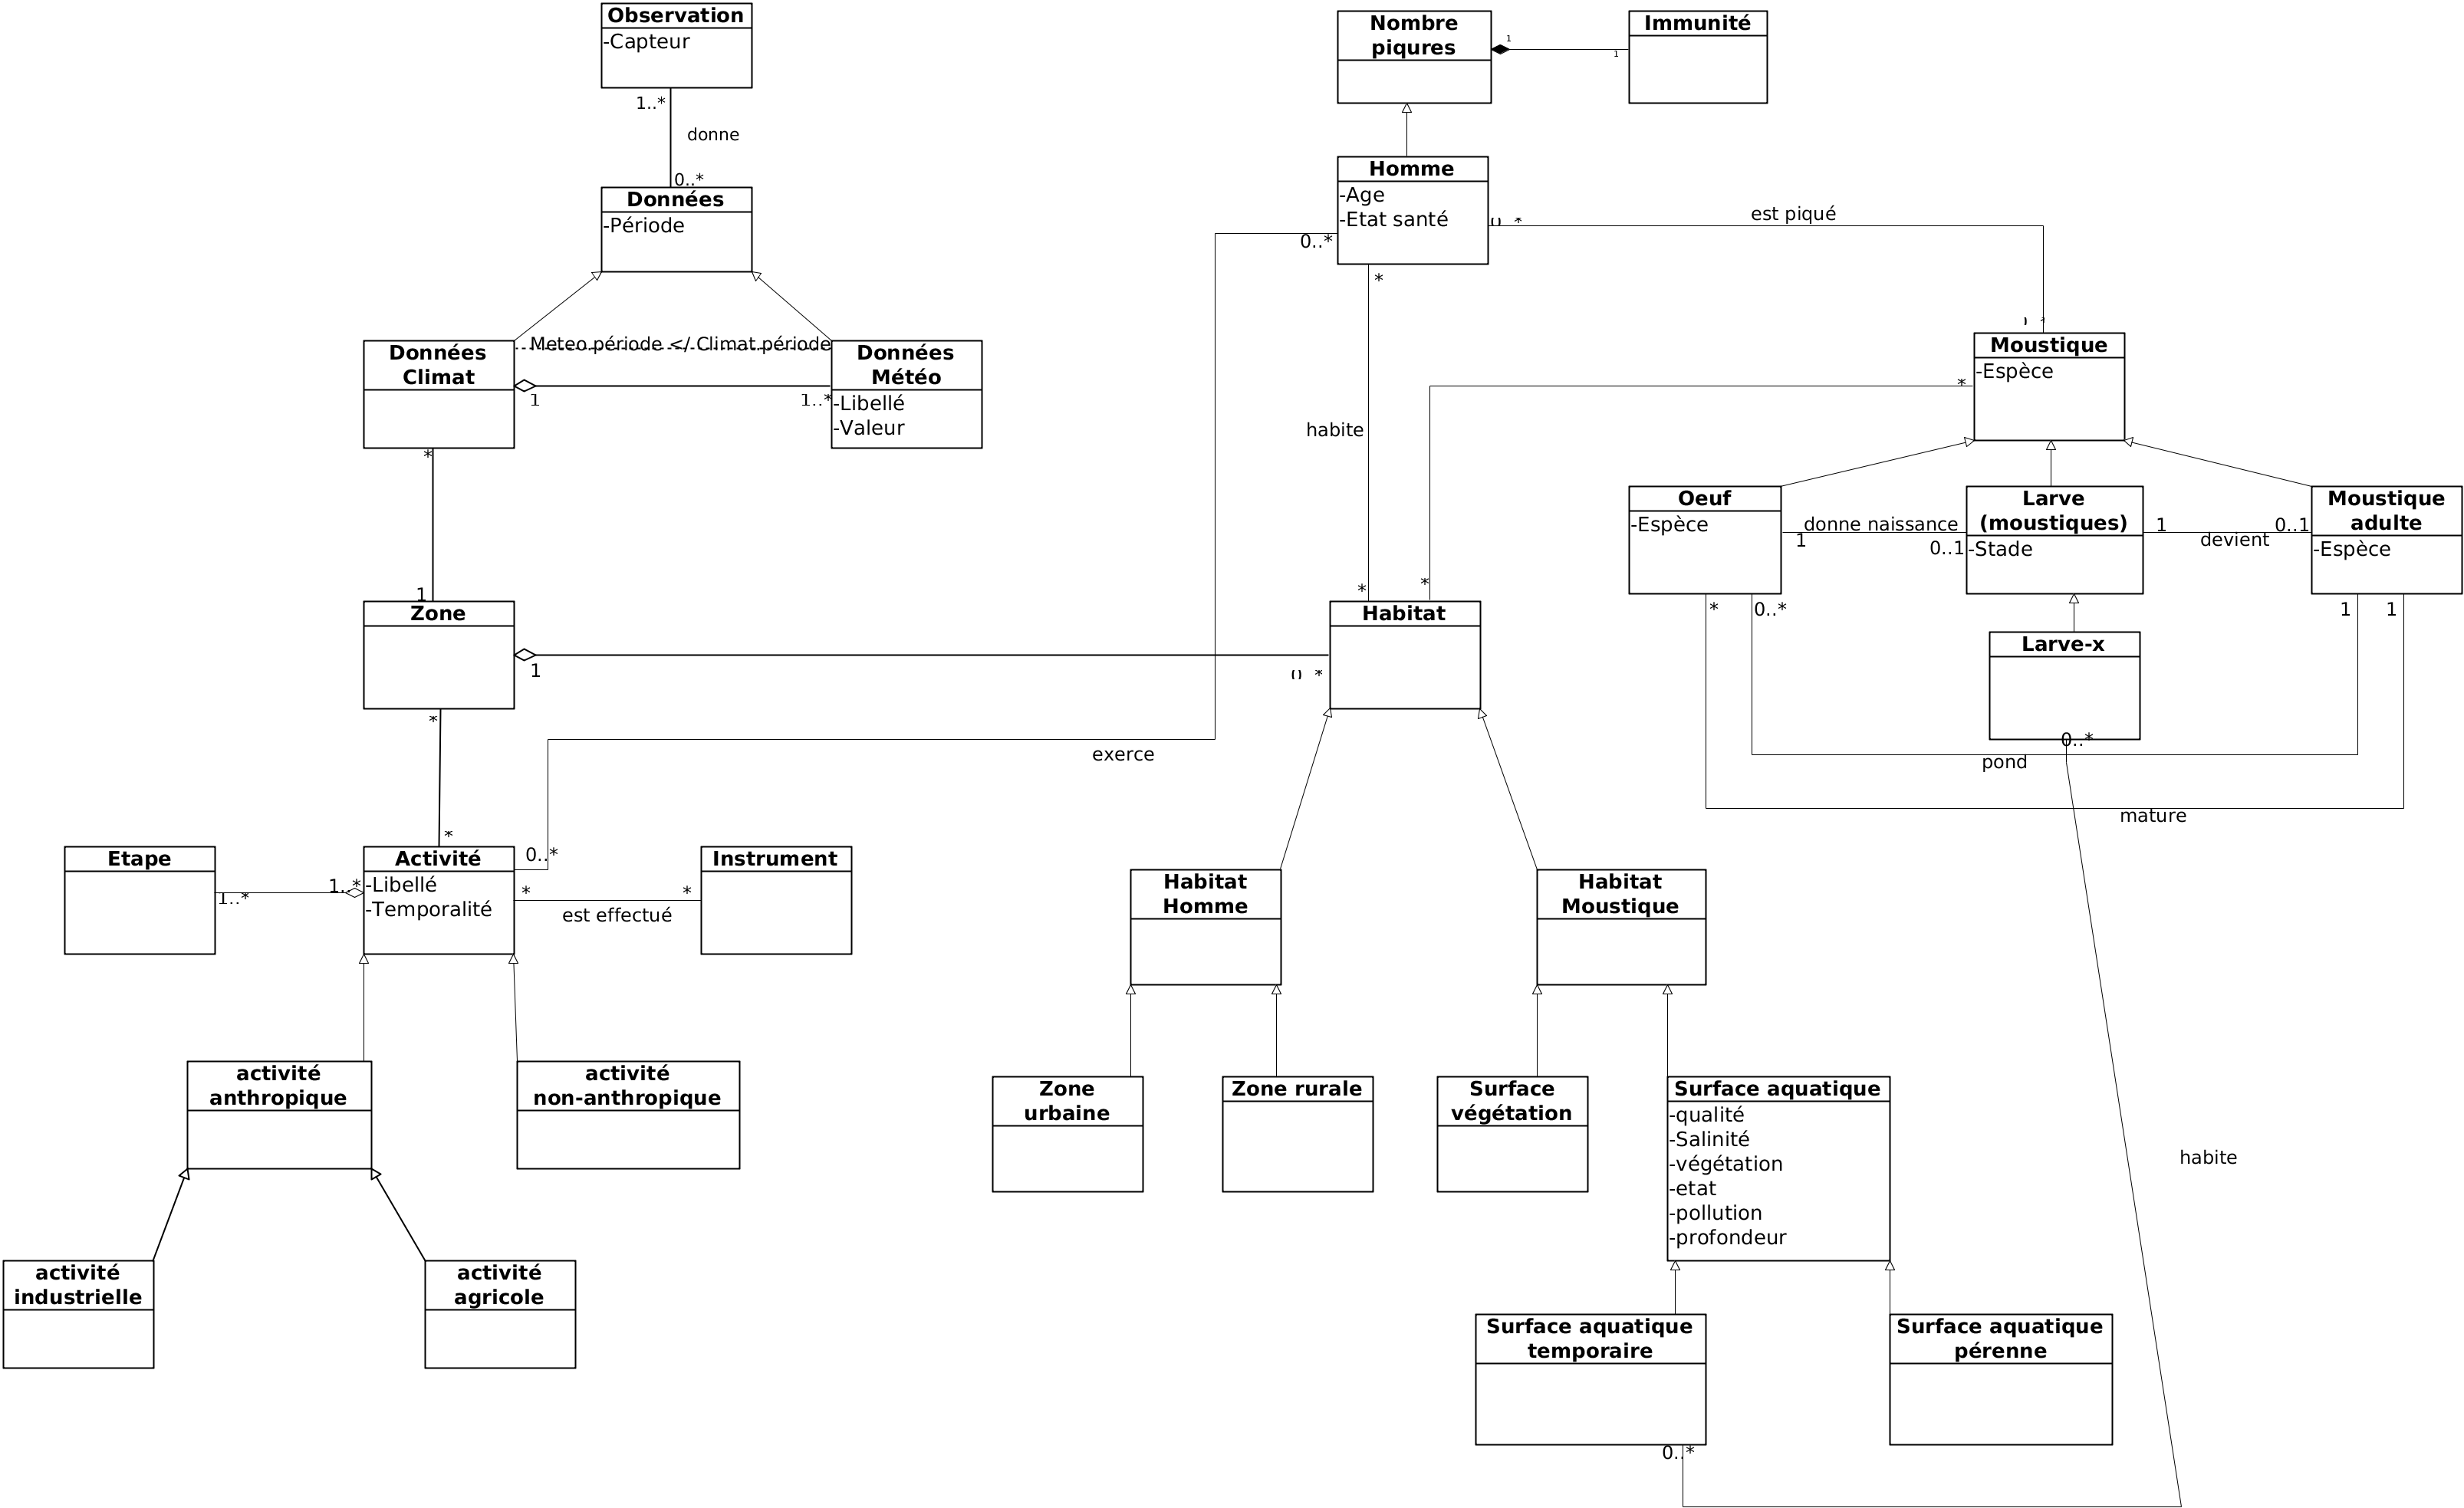
\includegraphics[width=23cm]{DiagrammeUML}\\
\caption{\label{UML_malaria} Modèle conceptuel UML des éléments nécessaires à l'élaboration des indicateurs}
\end{figure}
\end{landscape}

\subsubsection{Précision modèle conceptuel}

Des observations ont été effectuées sur un territoire (dans notre cas le village de Bandiagara au Mali). Les \textbf{observations} sont réalisées à l'aide de capteurs, comme par exemple des satellites. Une observation crée des \textbf{données} pour une période donnée. Dans le contexte de ce travail, il faut différencier les \textbf{données climat} et les \textbf{données météo}, c'est-à-dire que nous allons plutôt utiliser des données météo, qui elles font partie de données climatologiques. Les données climatologiques (généralement 30 ans) sont enregistrées sur une période plus longue, pour définir les grands principes du climat sur un territoire. Une donnée climatologique comprend donc plusieurs données météo, par exemple la température moyenne sur le territoire pendant le mois de Janvier 2008.
Une donnée climatique correspond à une \textbf{zone} définie. Sur cette zone sont exercées des \textbf{activités}. Ces activités sont effectuées à l'aide d'\textbf{instruments}. Une activité se divise en plusieurs étapes et peut être de type \textbf{anthropique} ou de type\textbf{non-anthropique}. Une activité anthropique est une activité relative à l'activité de l'homme comme par exemple les activités industrielles ou agricoles.

Les hommes habitent des \textbf{zones rurales} ou des \textbf{zones urbaines}. Cette différenciation est très importante, par exemple en zone urbaine le risque d'être infecté par le paludisme est beaucoup plus faible qu'en zone rurale car généralement les \textbf{eaux de surface} sont trop polluées pour abriter le moustique.
Les moustiques ont besoin d'\textbf{habitats} et d'endroits pour pondre leurs œufs. Les \textit{larves} nécessitent des surfaces aquatiques. La qualité, la salinité etc. d'une surface d'eau, la pollution et la profondeur jouent un rôle déterminant dans le cycle du développement de la larve. Généralement dans les zones à risque les \textbf{surfaces aquatiques pérennes} sont trop polluées et ne permettent pas le développement du moustique. Ainsi, un des facteurs de risque majeurs du paludisme est la présence de \textbf{surfaces aquatiques temporaires} car elles servent de lieu de pontage des œufs de moustique jusqu'à ce que les larves deviennent des moustiques. Les \textbf{moustiques adultes} généralement habitent des surfaces de végétation.
Finalement les moustiques piquent les hommes. En fonction des nombres de piqures, de l'âge de l'homme et de son état de santé, l'homme développe une certaine immunité. Un \textbf{homme} porteur du parasite peut également infecter un moustique non infecté auparavant.

\subsection{Données disponibles}

Nous disposons d'un certain nombre de données et d'informations relatives au territoire d'étude (Ville de Bandiagara). Ces données ont été extraites par Nadine Dessay à partir d'une image à très haute résolution Quick Bird (précision...). Les données correspondent aux facteurs de risque suivants :\\
\begin{itemize}
\item Végétation
\item Eau
\item Bâtiments\\
\end{itemize} 

En plus, nous disposons de données statistiques (données matricielles) issu d'un recensement de la population de la ville de Bandiagara en 2004 (14133 habitants) et des limites administratives des quartiers obtenues à partir de relevés GPS sur le terrain.\\

\subsection{Modèle UML simplifié}

A partir des données disponibles, nous avons élaboré un modèle conceptuel simplifié qui a servi comme point de départ pour la conceptualisation et l'élaboration de la chaîne de traitements. La partie concernant les activités effectuées sur une zone donnée a été écartée du modèle car il sera quasiment impossible de disposer de ces données. Il en est de même pour le cycle de vie du moustique qui n'interviendra pas dans les traitements.
Finalement le modèle suivant a été retenu :

\begin{center}
\begin{figure}[h] \centering
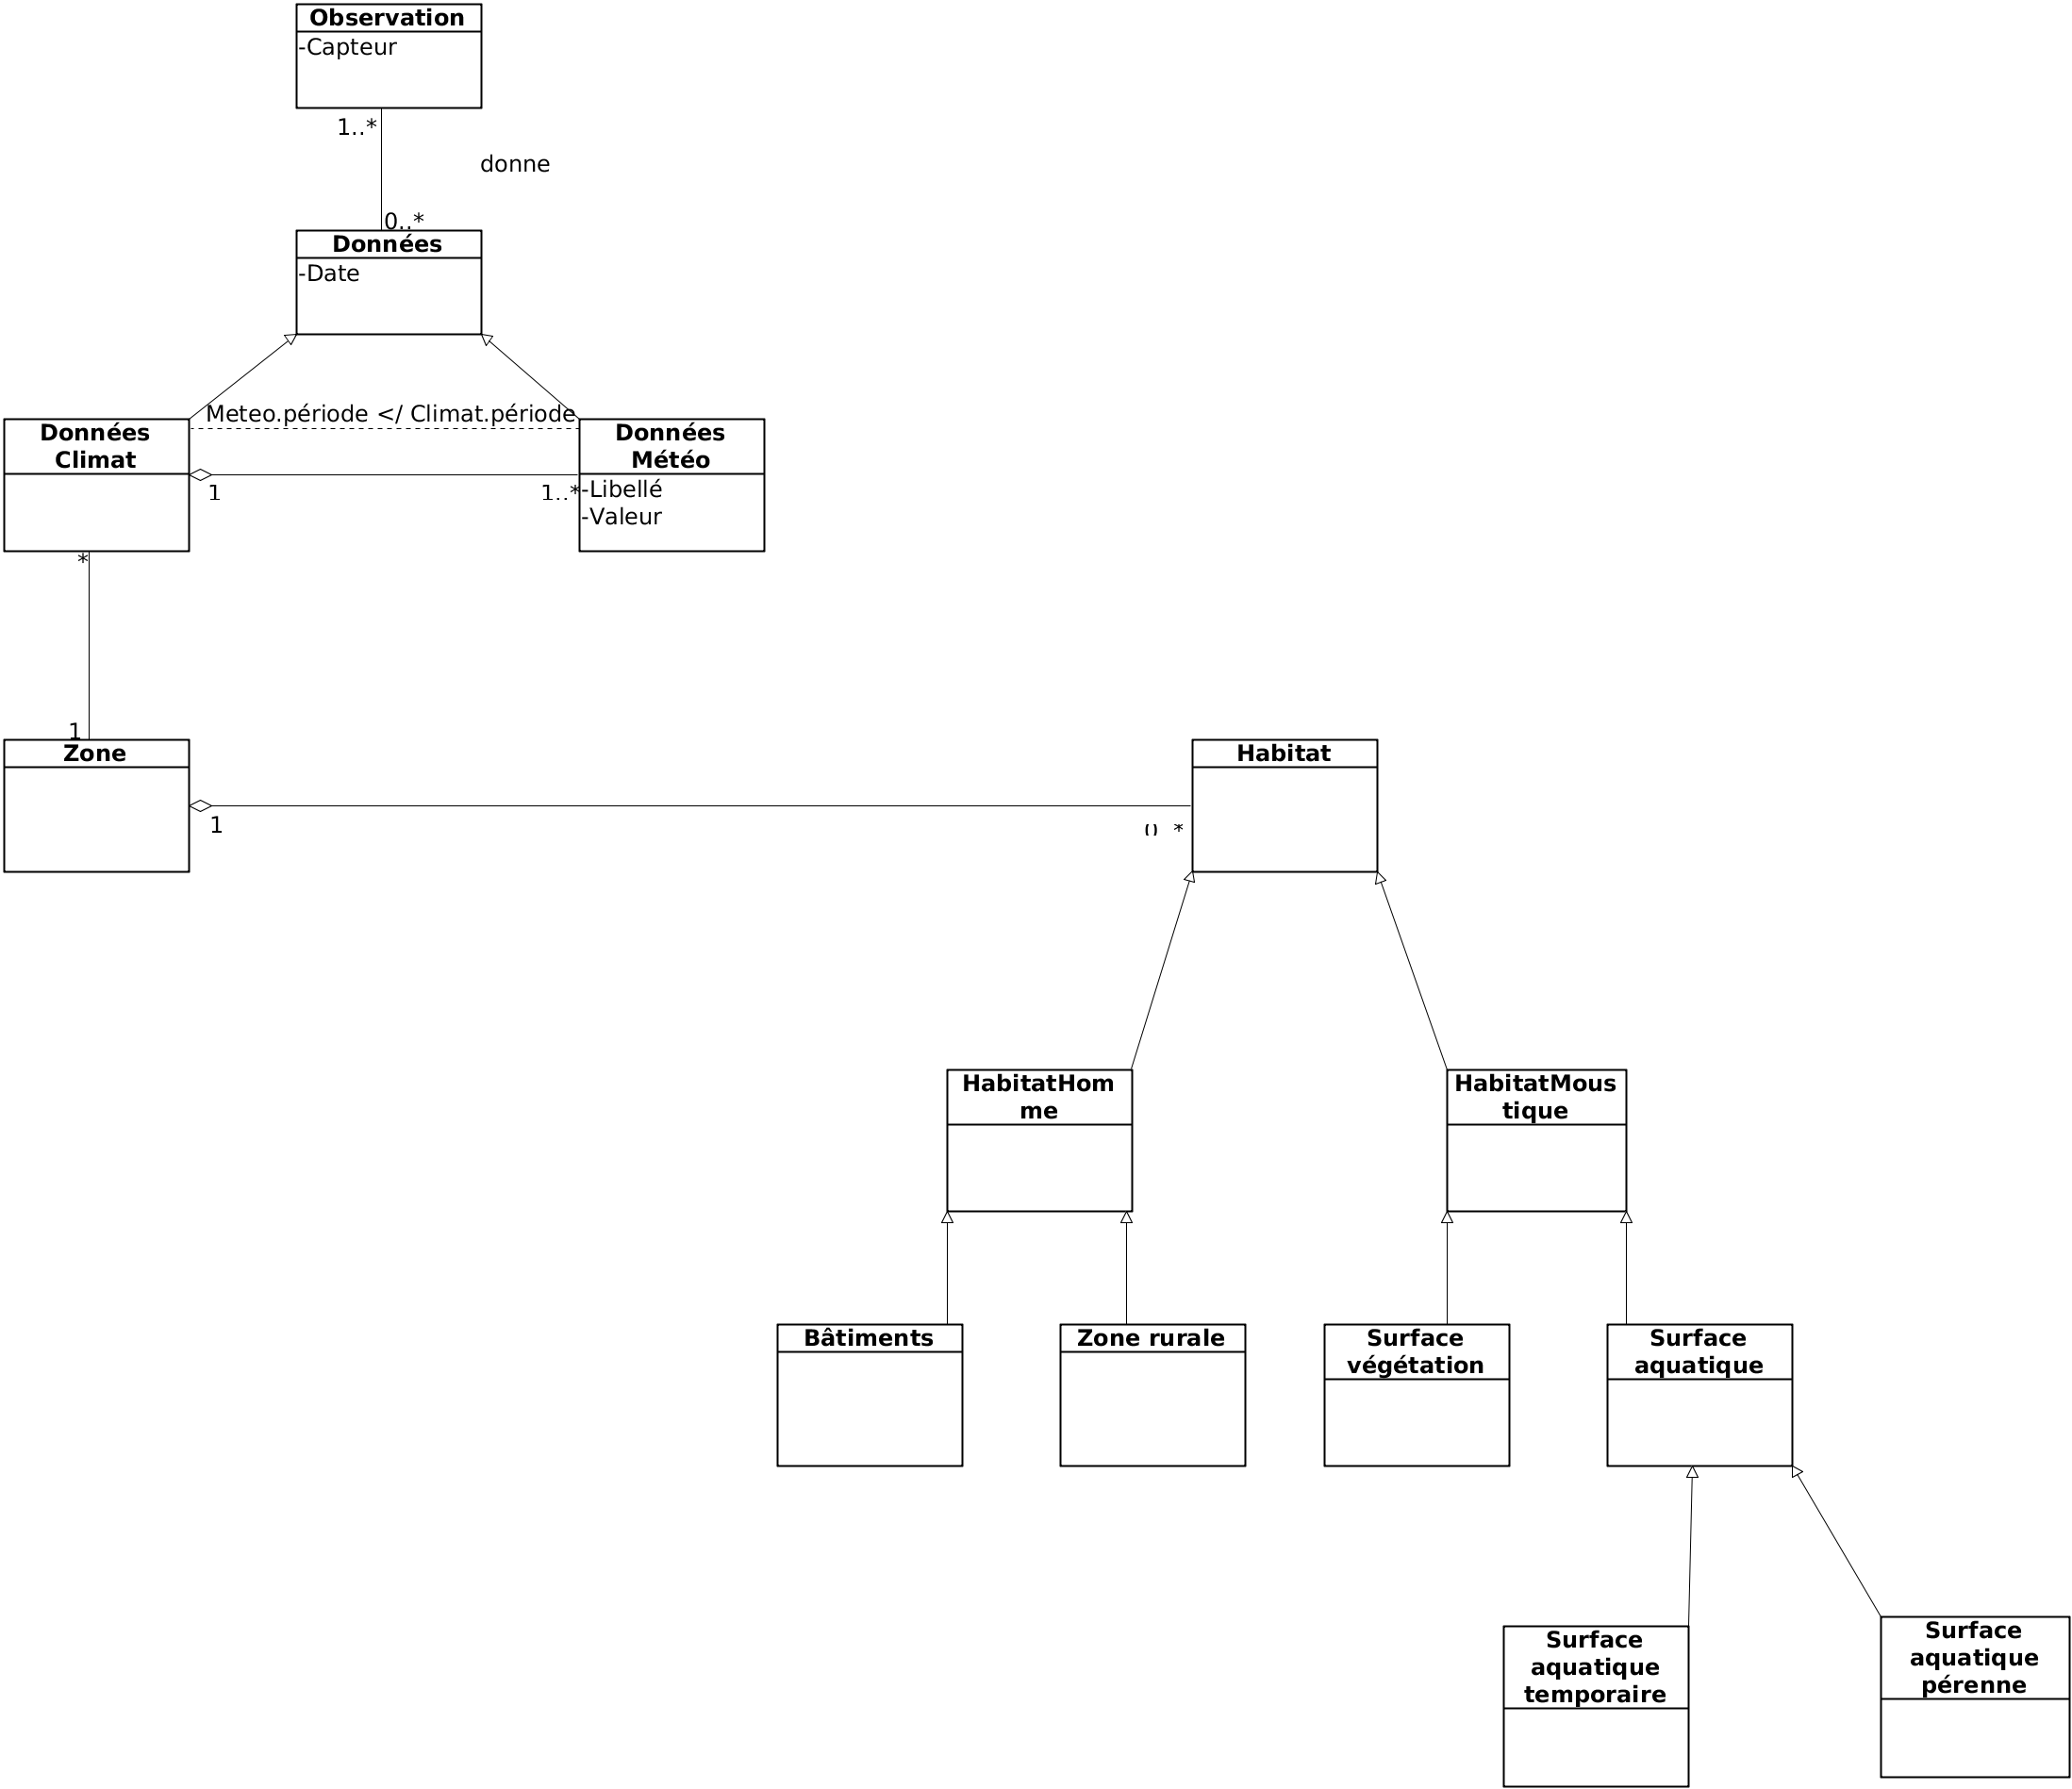
\includegraphics[width=14cm]{DiagrammeUMLsimplif.png}\\
\caption{\label{UMLSimplif_malaria} Modèle UML simplifié des indicateurs du paludisme}
\end{figure}
\end{center}

Le modèle conceptuel simplifié comprend les catégories de risques suivantes : \\
\begin{itemize}
\item Données climatologiques (précipitations, température etc). => aléa
\item Présence de surface d'eau (temporaires ou pérennes) => aléa
\item Présence de surface végétales => aléa
\item Habitations humaines => vulnérabilité\\
\end{itemize}

La présence humaine est indispensable pour qu'il y ait un risque (vulnérabilité) dans une zone. La présence de bâtiments a été retenue comme facteur de risque lié à cette présence humaine. Les surfaces végétales et les surfaces d'eau sont retenues respectivement  comme lieu d'habitation potentiel pour les moustiques anophèles et pour les larves de moustiques anophèles.

Ce modèle UML simplifié nous a servi de base pour conceptualiser le raisonnement de construction des indicateurs et la définition des traitements.

%Introduire le fait que les observations (terrain / satelite) ont été faites sur le territoire concerné, qu'elles concernent le moustique, l'habitat humain et la végétation/surface aquatique, éventuellement les données climatiques. Ces observatiosn vont être le point de départ de la chaîen de traitments à effectuer. 

%\subsection{Indicateurs}

\section{Raisonnement}

A partir des données disponibles, du modèle conceptuel simplifié et en collaboration avec des experts dans le domaine de l'environnement-santé et de la télédétection le raisonnement nous a permis de définir les traitements nécessaires pour l'élaboration de cartes de risque du paludisme. Nous nous sommes basés sur les travaux réalisés par Nadine Dessay. Une fois les traitements nécessaires définis nous nous sommes intéressés à la conceptualisation de l'enchaînement des traitements et des données. Cette partie est indispensable pour comprendre le futur fonctionnement de la chaîne de traitements.\\

\newpage

De façon très schématique le fonctionnement de la chaîne de traitements correspond au modèle suivant:\\


\begin{center}
\begin{figure}[h] \centering
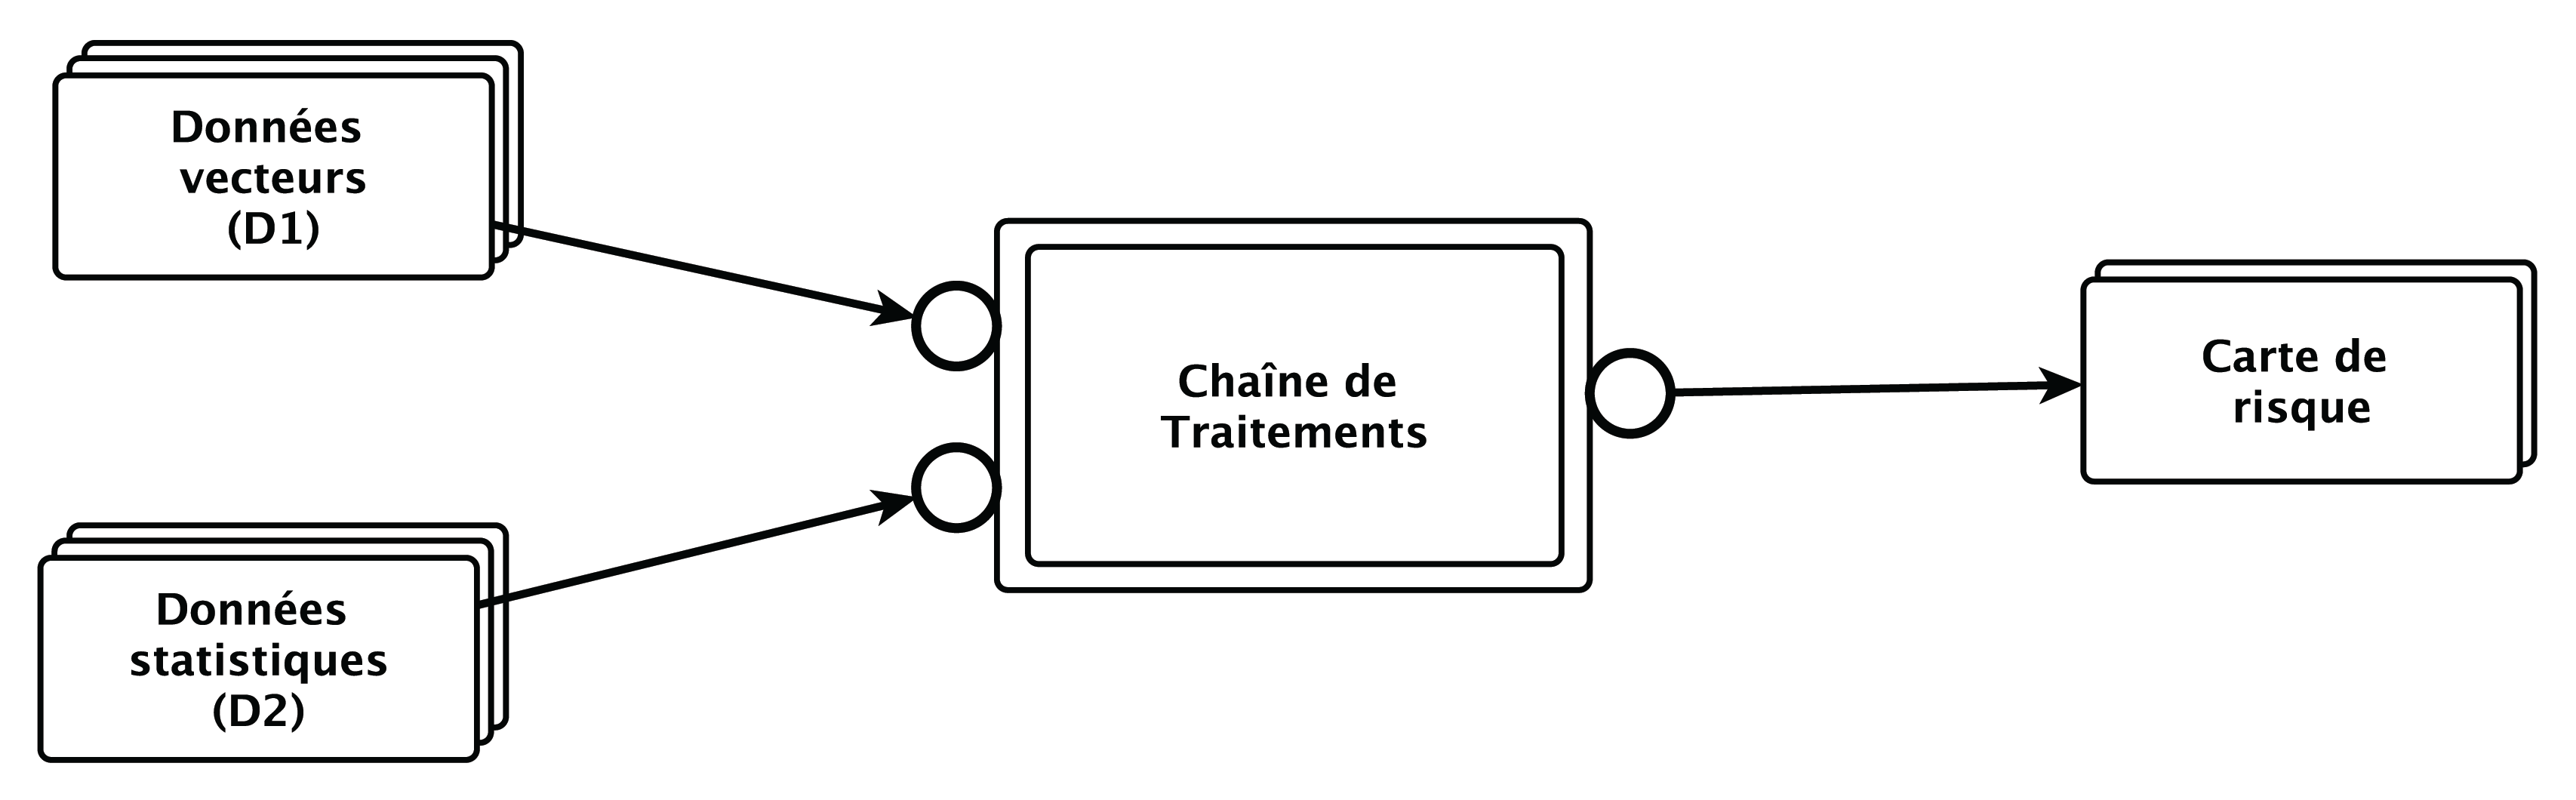
\includegraphics[width=12cm]{Traitement1.png}\\
\caption{\label{Traitements1} Description générale de la chaîne de la chaîne de traitements}
\end{figure}
\end{center}

Des traitements sont effectués sur des données de format vecteur et sur des données statistiques pour obtenir en sortie une carte de risque.
Nous expliquons dans un premier temps ce que fait un traitement et comment fonctionne une donnée. Ceci est fait à partir de \textbf{diagrammes de classes}.\\
Par la suite, des catégories de données et des catégories de traitements de la chaîne sont proposées à l'aide de \textbf{modèles conceptuels des hiérarchies}. Ceci permet de mieux comprendre le fonctionnement et les différentes étapes de la chaîne de traitements.\\


\subsection{Description des données et des traitements}

Nous allons décrire et expliquer les traitements réalisés au sein de la chaîne. Cette description peut être regroupée en 2 parties: \\

\begin{itemize}
\item La description globale de ce que fait un traitement
\item La description des données\\
\end{itemize}

Dans la suite de cette partie, nous expliquons successivement les deux aspects cités ci-dessus. Le modèle (\ref{TraitementModele}) qui suit décrit le fonctionnement d'un traitement.



\paragraph{1) Description globale de ce que fait un traitement\\}

Un traitement correspond à un propriétaire (contact), celui qui a respectivement développé ou défini le traitement. Chaque traitement correspond également à une ou plusieurs fonctionnalités et à une catégorie de traitements. Un traitement informatique comme par exemple l'édition nécessite les fonctionnalités comme par exemple ouvrir un fichier ou exporter un fichier. Un traitement correspond à diverses catégories de traitement qui pour nous ont été déterminées et nommées : pré-traitements, traitements et post-traitements. (cf. \citep{Lin2011})\\

Un traitement met en jeu trois types de données : des données d'entrée, des données de sortie et des données de paramétrage. Les données seront expliquées plus en détail dans le paragraphe (\ref{descrDonnes}) suivant.\\

Exemple d'un traitement: \textbf{shp2pgsql\\}
\begin{itemize}

\item Propriétaire: PostGIS / GDAL
\item Fonctionnalité(s): Transformation du format, Reprojection
\item Catégorie: Traitement
\item Donnée d'entrée: Fichier au format vecteur (shape)
\item Donnée en sortie: Fichier au format ".sql"
\item Donnée de paramétrage: postgis.sql, spatial\_ref.sql

\end{itemize}

\begin{figure}[H] 
\begin{center}
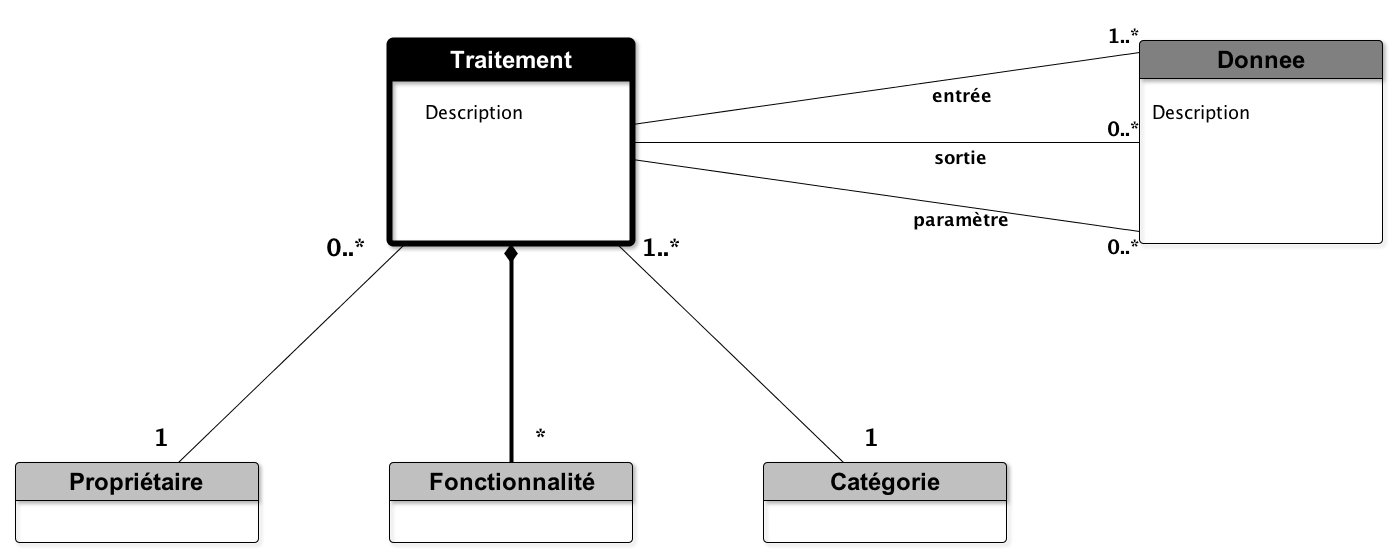
\includegraphics[width=15cm]{DescriptionTraitement5712.png}\\
\caption{\label{TraitementModele} Description du fonctionnement d'un traitement}
\end{center}
\end{figure}

\newpage
\paragraph{2) Description des données\\} \label{descrDonnes}

Décrire les traitements d'un système demande également de décrire les données utilisées. Une données correspond à une catégories de données, un  propriétaire et un format. (cf. \citep{ElKader2006}) \\

\begin{figure}[H] 
\begin{center}
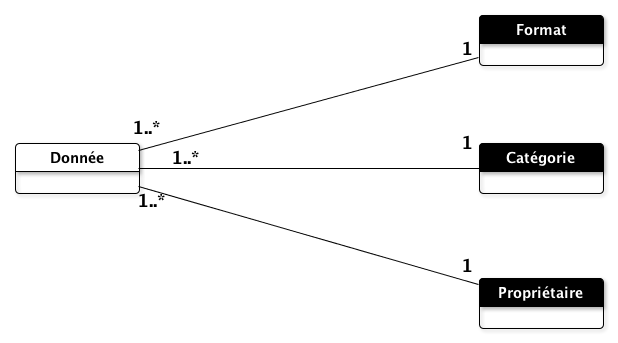
\includegraphics[width=9cm]{DescriptionDonnees}\\
\caption{\label{DescriptionDonnees} Description des données }
\end{center}
\end{figure}

Dans le contexte de ce travail, les formats de données utilisés sont les suivants : Format vecteur (fichiers de forme géoréférencés), format raster (images composites géoréférencés) et format tableur (statistiques). Ces données correspondent à des fonctionnalités comme par exemple la création de zones tampons. Chaque donnée est également caractérisée par un propriétaire (contact) et une catégorie de données. Nous pouvons regrouper les données utilisées, dans notre contexte, en deux catégories principales : les données issues de capteurs satellites et les données récoltées sur le sol (stations ou capteurs au sol).\\ 
%Une donnée correspond également à un type de données. Une donnée vecteur peut être par exemple de "type" ligne ou polygone. \\


Exemple de donnée: \textbf{b\_bati.shp}\\
\begin{itemize}

\item Propriétaire: Nadine Dessay
\item Catégorie: Raster
\item Format: vecteur (shape)

\end{itemize}

\newpage

\subsection{Les catégories de données et de traitements} \label{catdonnees}

\subsubsection{Les catégories de données}
Le modèle conceptuel des catégories de données (\ref{ModeleDonneesMin}) décrit de façon formelle les catégories de données qui sont utilisées par la chaîne de traitements.\\

\begin{figure}[H]
\begin{center}
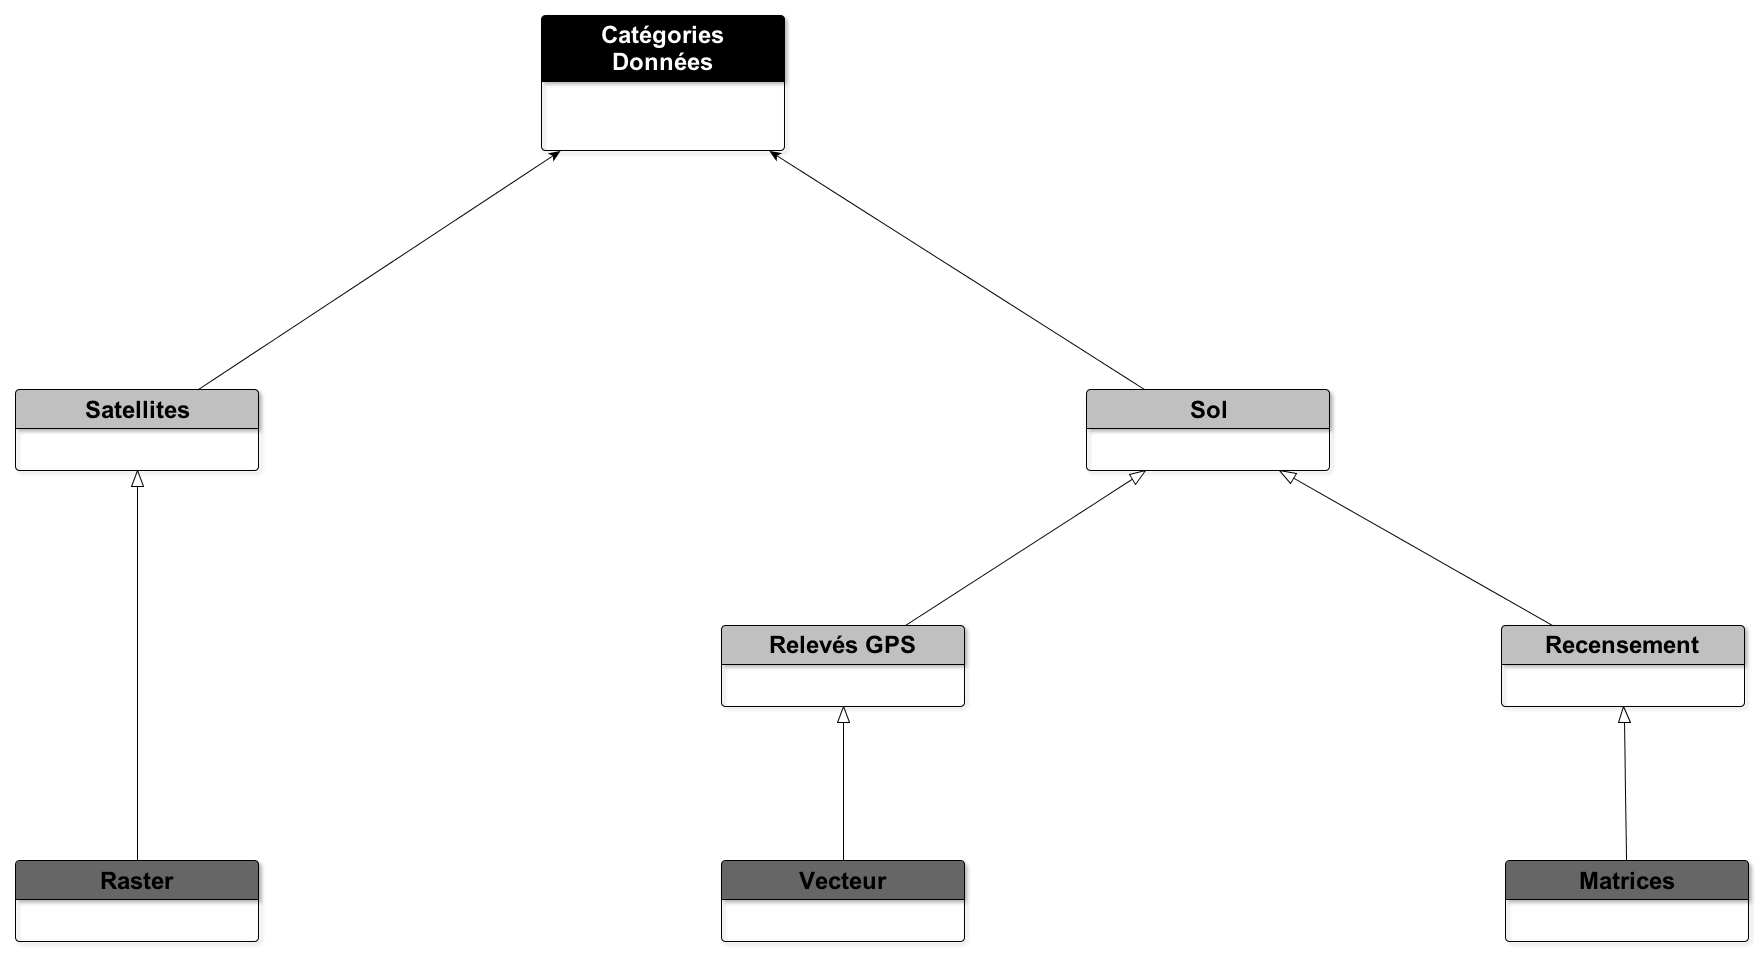
\includegraphics[width=16cm]{ModeleDonneesMin}\\
\caption{\label{ModeleDonneesMin} Modèle conceptuel des catégories de données de la chaîne de traitements}
\end{center}
\end{figure}


Les données de la chaîne de traitements sont issues de sources diverses. Les \textbf{données issues de satellites} correspondent aux données obtenues à partir de satellites (passifs ou actifs).
Les \textbf{données issues du sol} sont les données qui proviennent de capteurs ou de toute autre source se situant sur le sol terrestre. \\

Les satellites produisent des \textbf{images raster}, à partir desquelles, en ayant recours à des traitements de télédétection, peuvent être extraites de nombreuses informations. Pour notre chaîne de traitements, les informations suivantes ont été extraites par des experts en télédétection (Nadine Dessay):\\

\begin{itemize}
\item Eau: Les surfaces d'eau
\item Végétation: Les arbres etc.
\item Urbanisation: Bâtiments\\
\end{itemize}

Les données récoltées sur le \textbf{sol} peuvent correspondre à différentes catégories. Par exemple, une station météo peut fournir des données de catégorie vecteur ou raster. Des relevés GPS fournissent des vecteurs. Des statistiques (catégorie matrices) sont obtenues à partir de recensements de population par exemple.


\subsubsection{Les catégories de traitements}



Nous proposons trois grandes catégories de traitements: Les \textbf{pré-traitements}, les \textbf{traitements} et les \textbf{post-traitements}.
La catégorie des pré-traitements recouvre l'ensemble des opérations qui préparent les données pour qu'elles puissent être traitées. Dans le cadre de ce travail il est nécessaire de stocker les données et d'effectuer des requêtes SQL afin de sélectionner les données à en fonction des traitements.\\

La catégorie des traitements recouvre les traitements proprement dits, c'est à dire les traitements qui vont créer ou modifier des données. Cette catégorie présente trois sous-catégories : les traitements \textbf{statistiques} ,les traitements \textbf{d'analyse spatiale} et les traitements de \textbf{transformation}. \\

Les traitements statistiques concernent les calculs de densités de population, de densité de points et le calcul de la taille de cellule des couches raster.

Les traitements d'analyse spatiale sont les traitements géographiques sur les \textbf{fichiers de forme} (shape) (par exemple intersection entre deux fichiers de forme vecteurs).\\

Les traitements de transformation correspondent aux traitements qui modifient le format des données. Par exemple, pour insérer un fichier vecteur dans une base de données spatiale, il est nécessaire d'effectuer une transformation vers le format ".sql".

Les post-traitements concernent tout ce qui est représentation des résultats obtenus, par exemple une reclassification d'une image raster pour faire ressortir une information plus clairement.



\begin{figure}[H]
\begin{center}
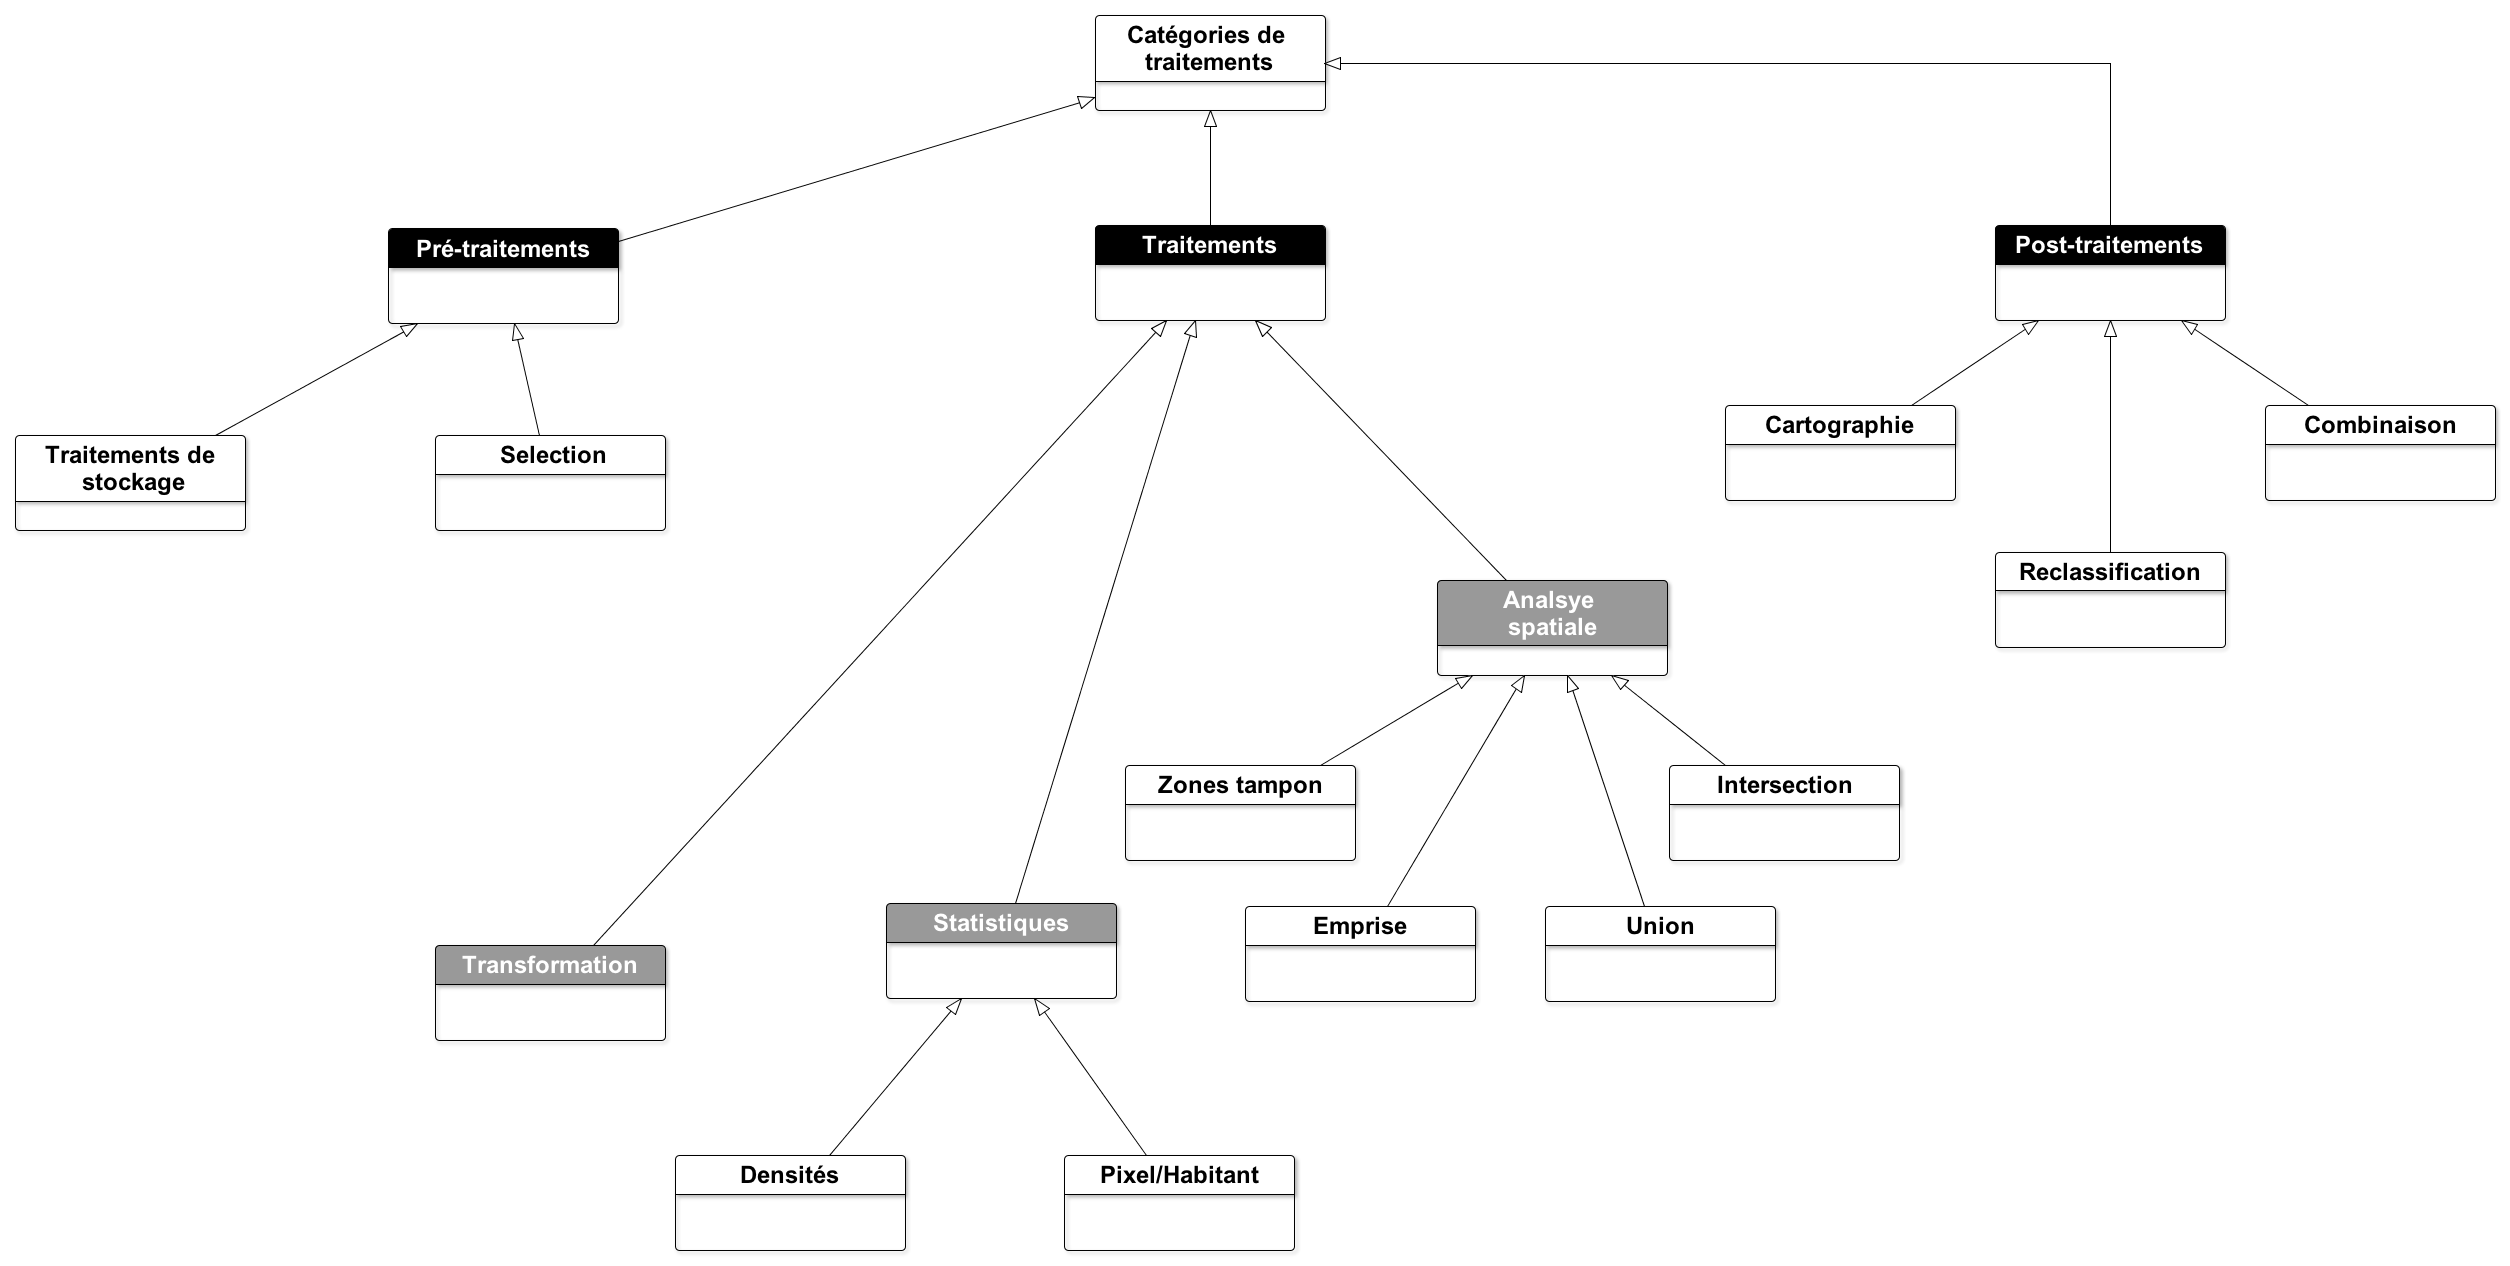
\includegraphics[width=16cm]{ModeleTraitements2}\\
\caption{\label{ModeleTraitements} Modèle conceptuel des hiérarchies de catégories de traitements de la chaîne de traitements}
\end{center}
\end{figure}



\subsection{Conceptualisation de la chaîne de traitements}

Le modèle conceptuel des traitements permet de représenter la dynamique de la chaîne de traitements, c'est-à-dire les opérations et traitements qui sont réalisées en fonction d'autres événements. 
Ce modèle permet donc de représenter et d'expliquer de façon conceptuelle le fonctionnement du système sans faire référence aux choix qui ont été réalisés (par exemple quelle librairie a été utilisée, quel langage informatique etc.). Le modèle explique donc les traitements qui sont effectués dans la chaîne mais il n'explique pas comment ils sont effectués.  \\

Pour illustrer les différentes opérations de la chaîne de traitements, nous allons détailler successivement comment se construit la chaîne de traitements à partir des descriptions précédentes et comment l'instanciation est réalisable à partir du modèle de départ (cf \ref{Traitement11})\\

%Pour faciliter la représentation des chaînes abstraites nous utiliserons le langage graphique proposé par Yuan Lin (\ref{LinGraph}). Les ports de données associés à un traitement abstrait ont pour objectif de distinguer les différents flux de données en terme d’entrée / sorties \citep{Lin2011}.



\subsubsection{Description générale}

Pour créer une carte de risque, il est nécessaire d'effectuer des traitements sur des données. Les données d'entrée correspondent à deux formats différents : format vecteur et format statistique. Ces données sont utilisées par la chaîne de traitements pour effectuer les traitements nécessaires pour cartographier le risque.\\


\begin{figure}[H]
\begin{center}
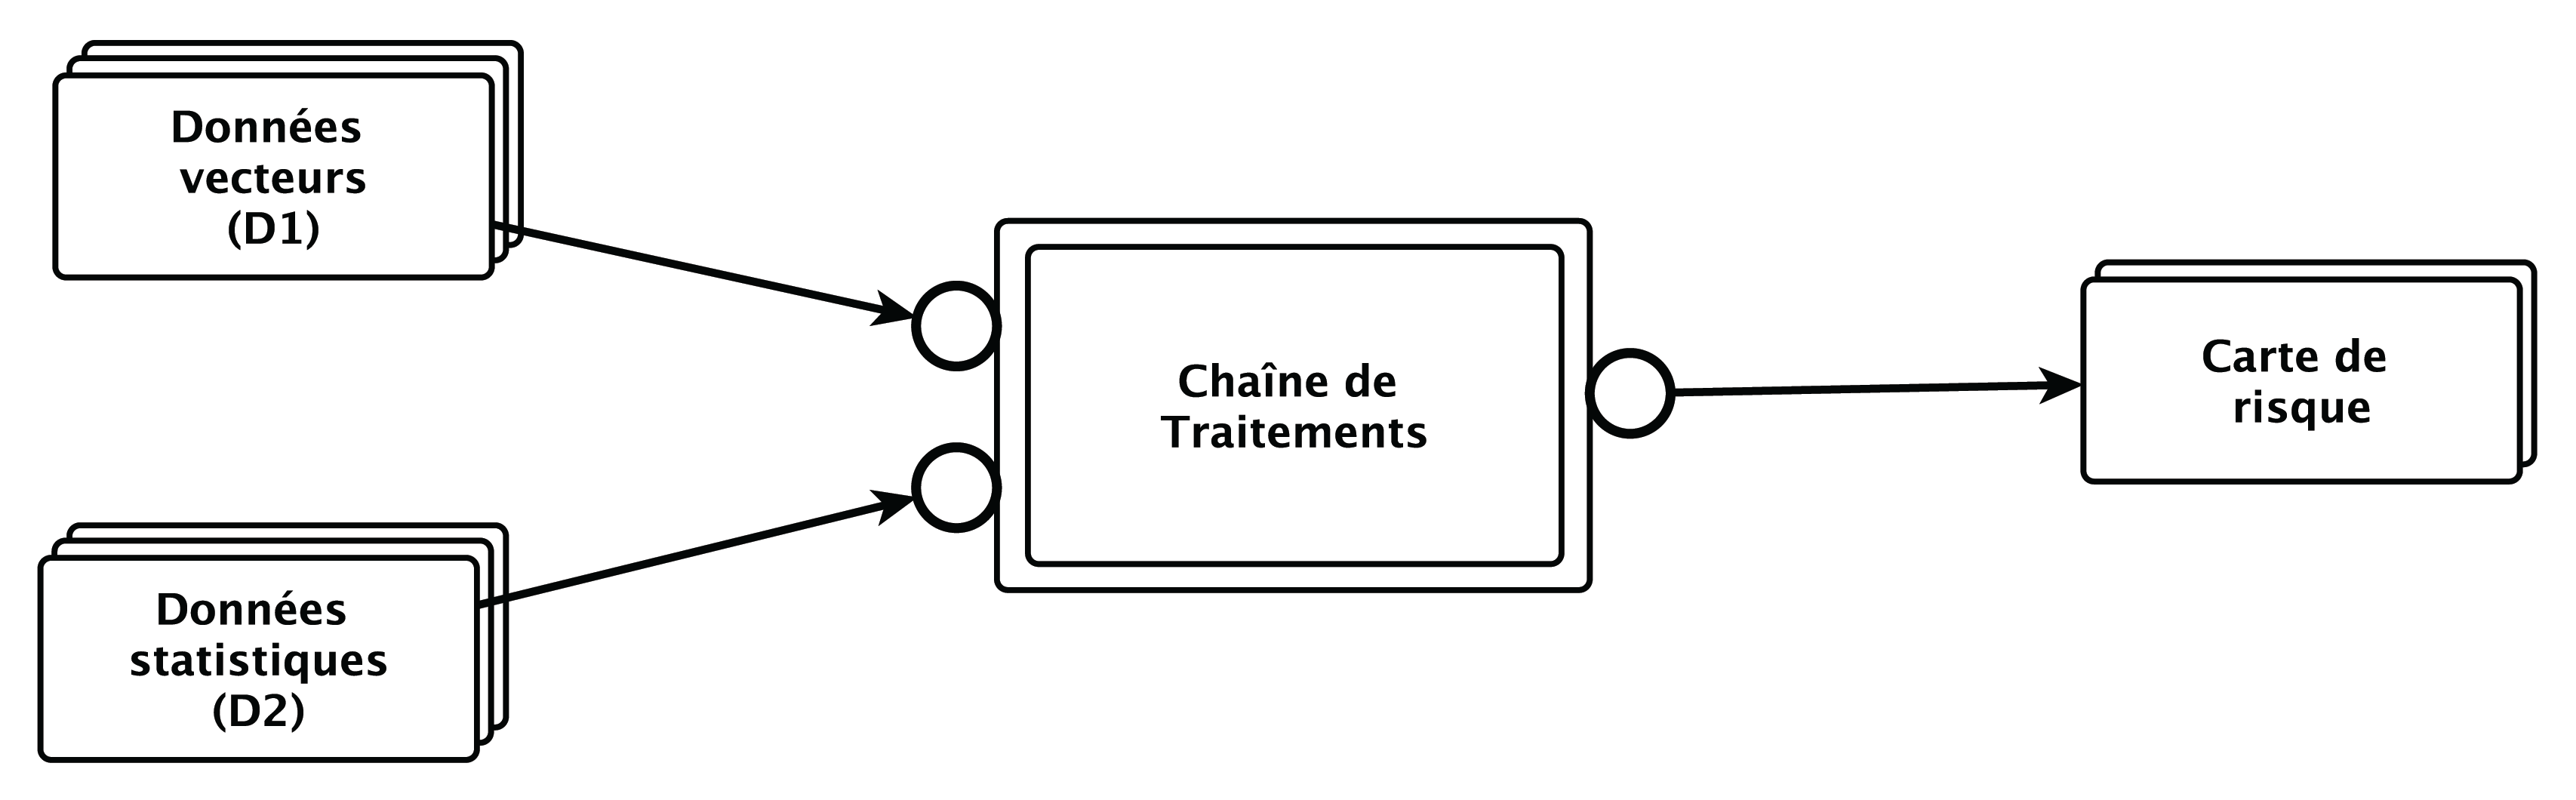
\includegraphics[]{Traitement1.png}\\
\caption{\label{Traitement11} Description générale}

\end{center}
\end{figure}




\subsubsection{Chaîne abstraite}

Dans un premier temps, les données vecteurs sont stockées (traitements de stockage) dans une base de données. Par la suite, des \textbf{sélections} permettent de définir précisément les données qui seront traitées lors de chaque traitement.\\

Le risque est la combinaison entre \textbf{l'aléa} et la \textbf{ vulnérabilité}. Deux grandes catégories de traitements sont effectuées : les traitements de vulnérabilité et les traitements d'aléa. Le traitement de risque permet de créer des cartes de risque.\\


\begin{figure}[H]
\begin{center}

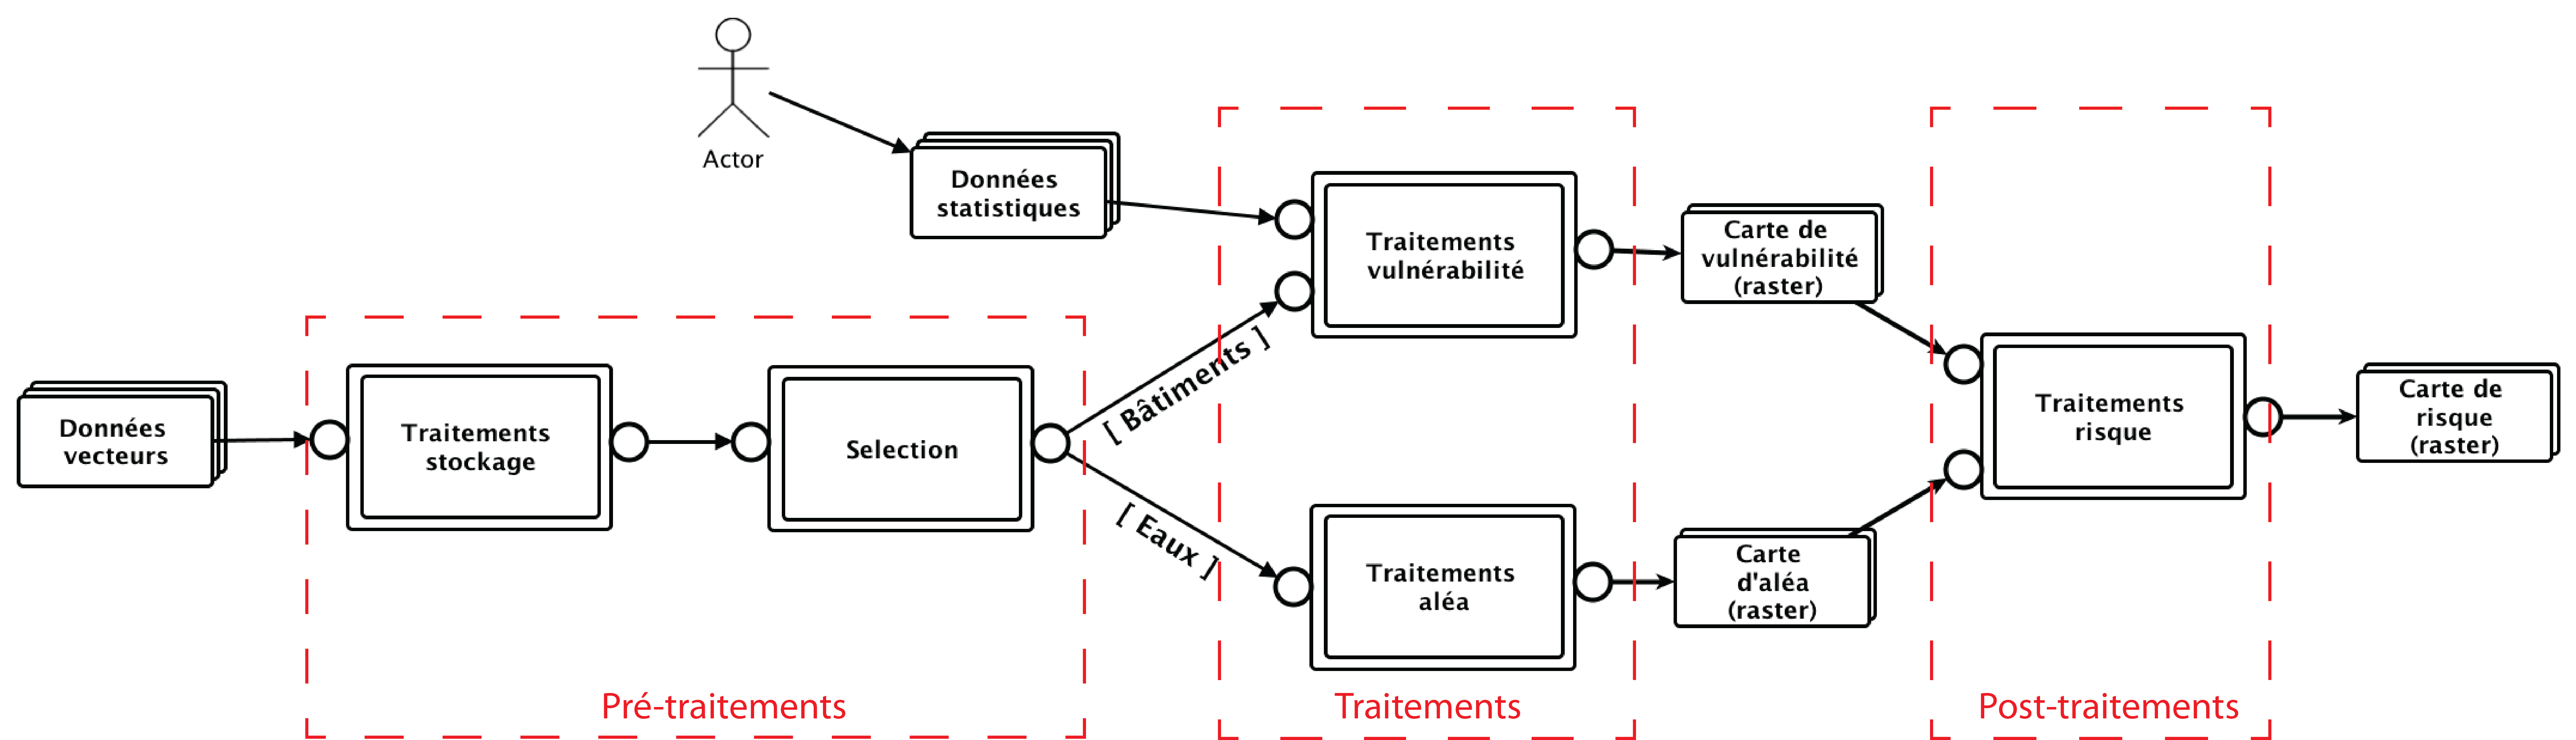
\includegraphics[width=15cm]{traitements2.png}\\
\caption{\label{Traitement12} Chaîne abstraite}
\end{center}
\end{figure}



\subsubsection{Traitements élémentaires de la chaîne de traitements}

Chaque donnée vectorielle stockée dans la base de données est dans un premier temps reprojetée (la projection de la base de données spatiale et de toutes les données insérées sera la même). Les données sont insérées dans une base de données spatiale (créée dans un \textbf{SGBD} au cours de l'exécution de la chaîne de traitements). Des requêtes SQL permettent de sélectionner (filtrer) les données à utiliser pour chaque traitement.\\

Les traitements de vulnérabilité correspondent à deux catégories de traitements : des traitements d'analyse spatiale et des traitements statistiques. La chaîne de traitements demande à l'utilisateur le nombre d'habitants de la zone d'études (= données statistiques). La chaîne de traitements crée une carte de vulnérabilité en combinant les deux catégories de traitement.\\

Les traitements d'aléa correspond à des traitements d'analyse spatiale sur les données "eau" (format vecteur). L'ensemble de ces traitements permettent de créer une carte d'aléa.\\

Les traitements de risque correspondent à la combinaison de la carte de vulnérabilité et de la carte d'aléa. La carte de risque est le résultat de l'ensemble des traitements.


\begin{figure}[H]
\begin{center}

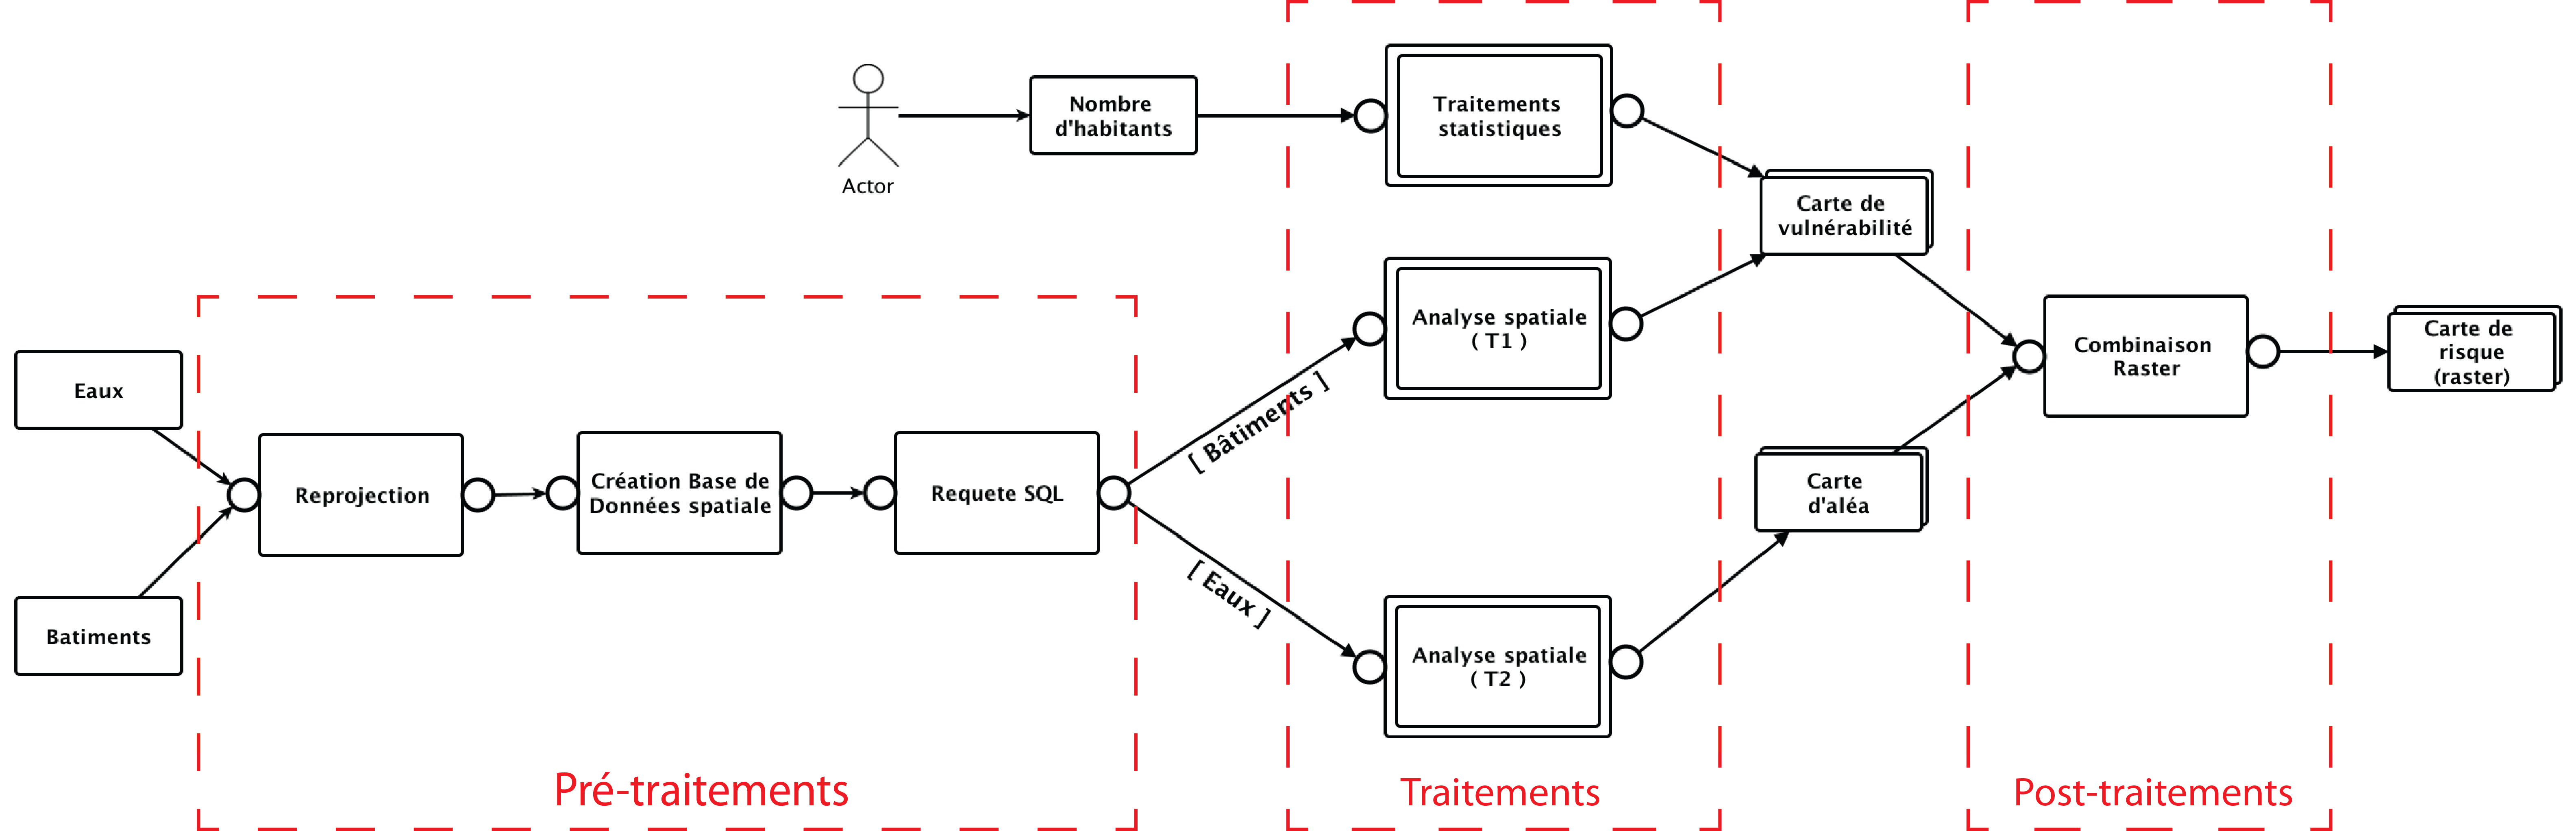
\includegraphics[width=15cm]{Traitements3.png}\\
\caption{\label{Traitement13} Chaine abstraire avec traitements élémentaires}
\end{center}

\end{figure}




\subsubsection{Chaîne de traitements de plus en plus détaillées}

Des requêtes SQL permettent de calculer la surface totale de la couche "bâtiments". A partir des informations saisies par l'utilisateur (nombre d'habitants), la chaîne calcule la densité de population de la zone d'étude. A partir de ces informations, la surface qu'occupe en théorie un habitant permet de calculer la taille théorique d'une cellule pour un habitant. La couche "bâtiments" est ensuite \textbf{rastérisée} en fonction de la taille de la cellule calculée par avant. Pour chaque \textbf{cellule de ce raster}, un point est créé et le calcul de la densité des points permet de créer une carte de vulnérabilité.\\

En ce qui concerne les traitements d'analyse spatiale de l'aléa, plusieurs traitements sont successivement effectués: définition de l'emprise de la zone d'étude, zone tampons autour de la couche "eaux" (400 et 600 mètres), union et intersection des résultats pour arriver à la création d'une carte d'aléa. (cf. Annexes)\\


\begin{figure}[H]
\begin{center}

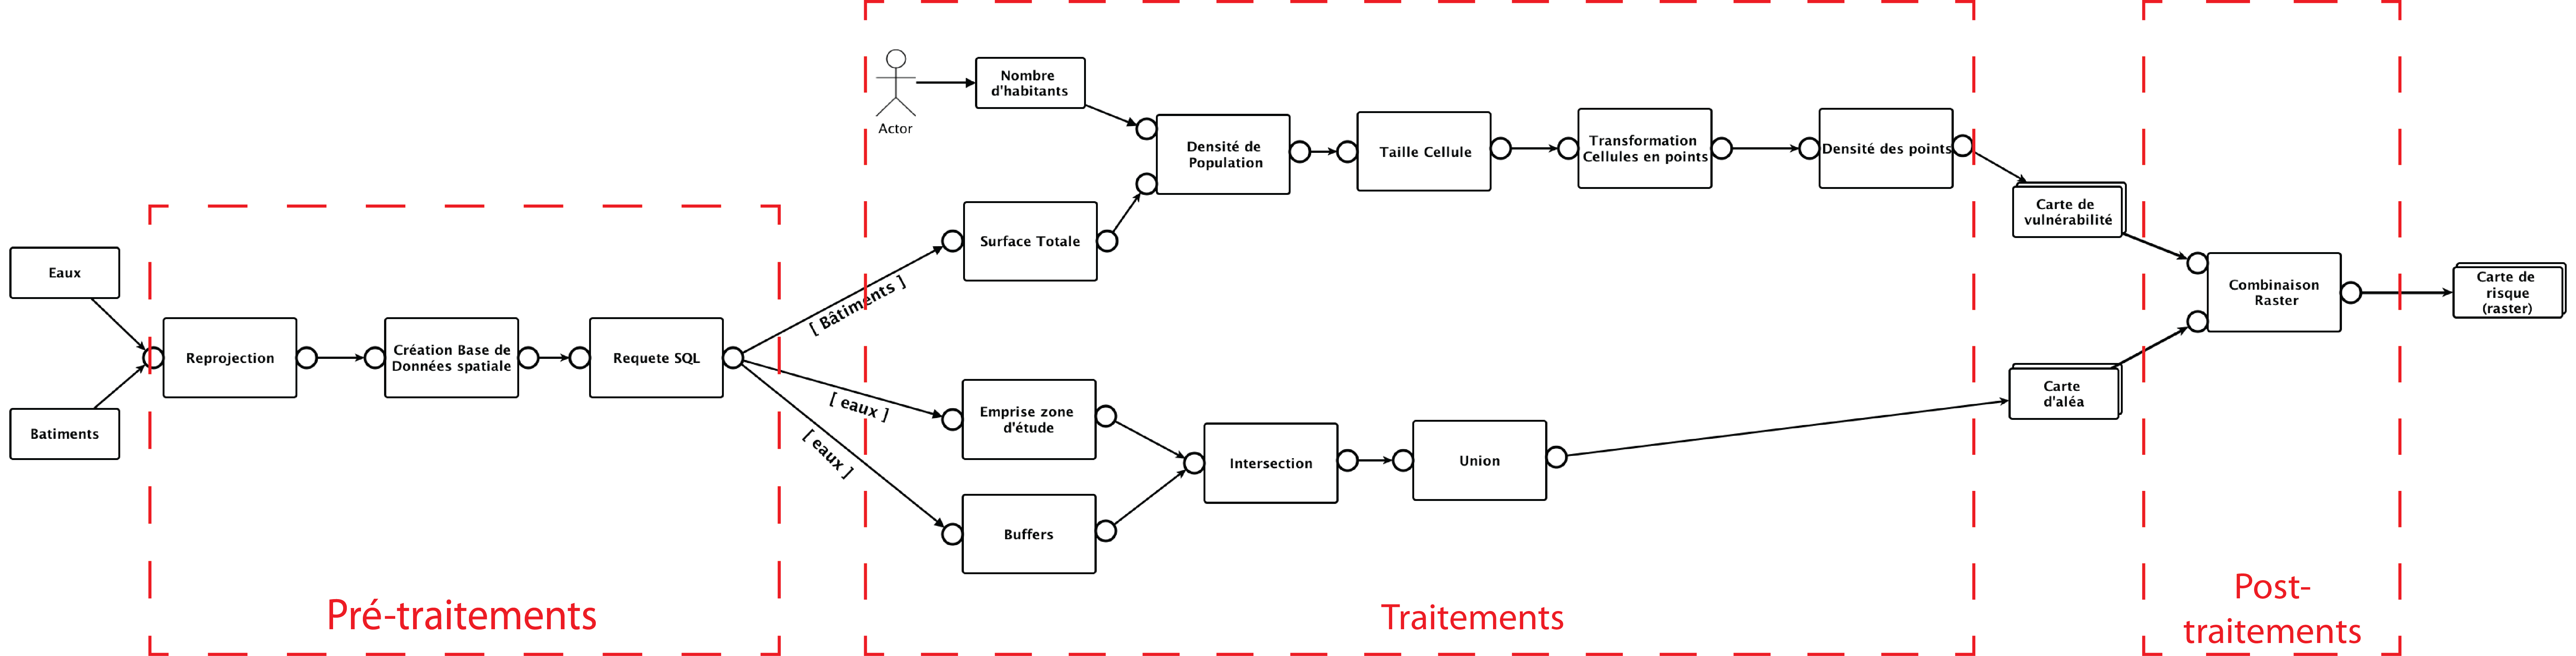
\includegraphics[width=15cm]{Traitement4.png}\\
\caption{\label{Traitement14} Chaîne de traitements de plus en plus détailée}
\end{center}
\end{figure}

\subsubsection{Chaîne de traitements instanciée}


\begin{figure}[H]
\begin{center}

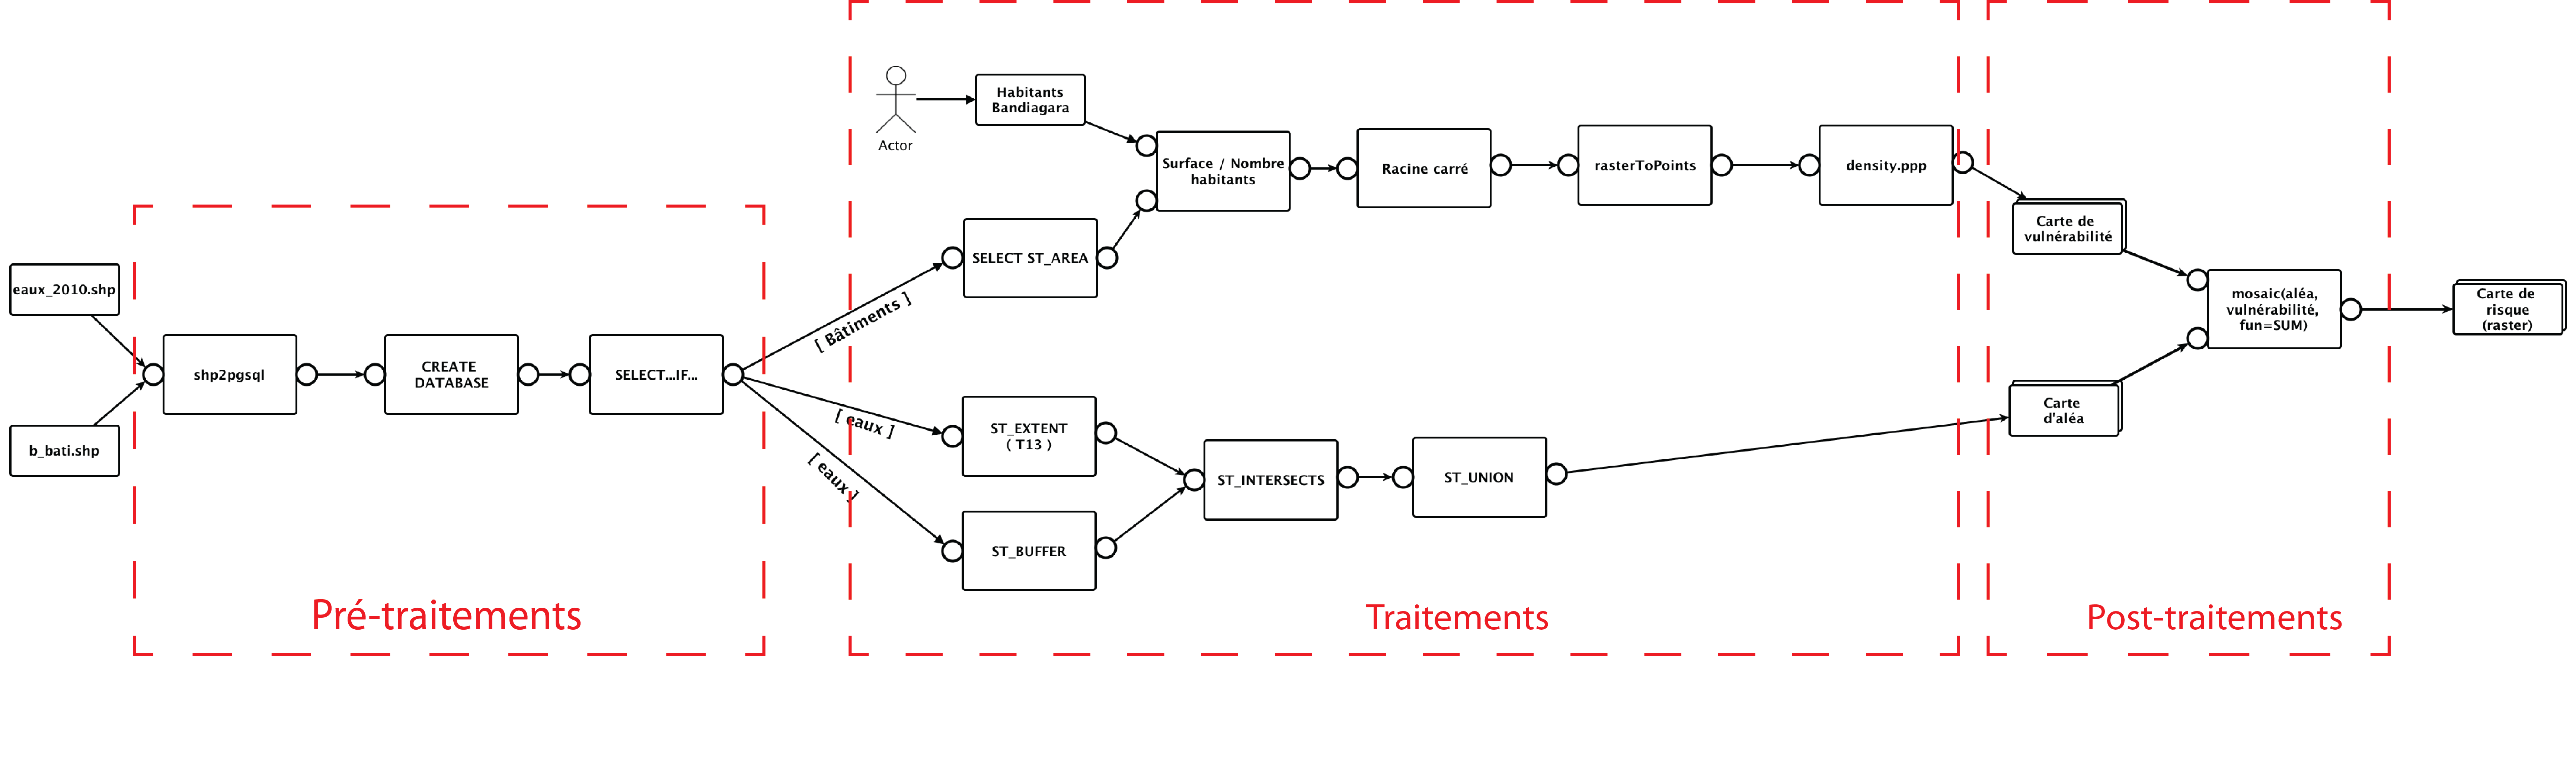
\includegraphics[width=15cm]{chaineinstanc.png}\\
\caption{\label{traitementsInstancie} Chaîne de traitements fermée instanciée}
\end{center}
\end{figure}

Nous utilisons pour l'exécution de la chaîne de traitements fermée deux fichiers de données en entrée: "b\_bati.shp" et "arbres.shp". La fonctionnalité PostGIS "shp2pgsql" permet de transformer et de reprojeter les deux données. Une base de données spatiale est créé et les données sont insérées dans cette base de données. Des requêtes SQL (select...if...) permettent de sélectionner (filtrer) les données nécessaires pour les différents traitements (par exemple "b\_bâti" pour les traitements de vulnérabilité). Les différentes fonctionnalités PostGIS comme "ST\_AREA" (surface d'une couche) ou "ST\_INTERSECTS" (intersection) ainsi que d'autre fonctionnalités R comme par exemple "density.ppp" permettent d'effectuer les traitements souhaités (cf. Annexes). Finalement, la fonctionnalité R "mosaic(...)" permet de combiner la carte de vulnérabilité et la carte d'aléa. 

\section{Conception}

Pour valider sur le plan opérationnel notre approche, nous avons réalisé deux types d'outils. Dans un premier temps, nous avons développé une chaine entièrement automatisée de traitements. L'utilisateur choisit les données d'entrée et la chaîne effectue automatiquement tous les traitements nécessaires pour la création d'une carte de risque. \\

Dans un second temps, nous avons développé un logiciel ouvert, l'utilisateur peut ainsi choisir les traitements qu'il souhaite effectuer.\\

Dans cette partie du travail, nous présentons l'implémentation des deux outils, respectivement l'architecture informatique des deux outils. Les librairies et bibliothèques utilisées sont présentées en Annexe.


\subsection{Architecture informatique de la chaine de traitements et du logiciel ouvert}

Le prototype de la chaîne de traitements et le logiciel ouvert appellent les fonctionnalités des outils PostgreSQL / Postgis (via le JDBC PostgreSQL) et R (via RCaller) via le langage Java. Le schéma suivant explique de façon très simplifiée l'architecture informatique des deux outils. Les deux outils peuvent également se connecter à une bas de données distante. Les autres composants de l'architecture doivent être installés en local sur la machine de l'utilisateur.\\

\begin{figure}[H]
\begin{center}
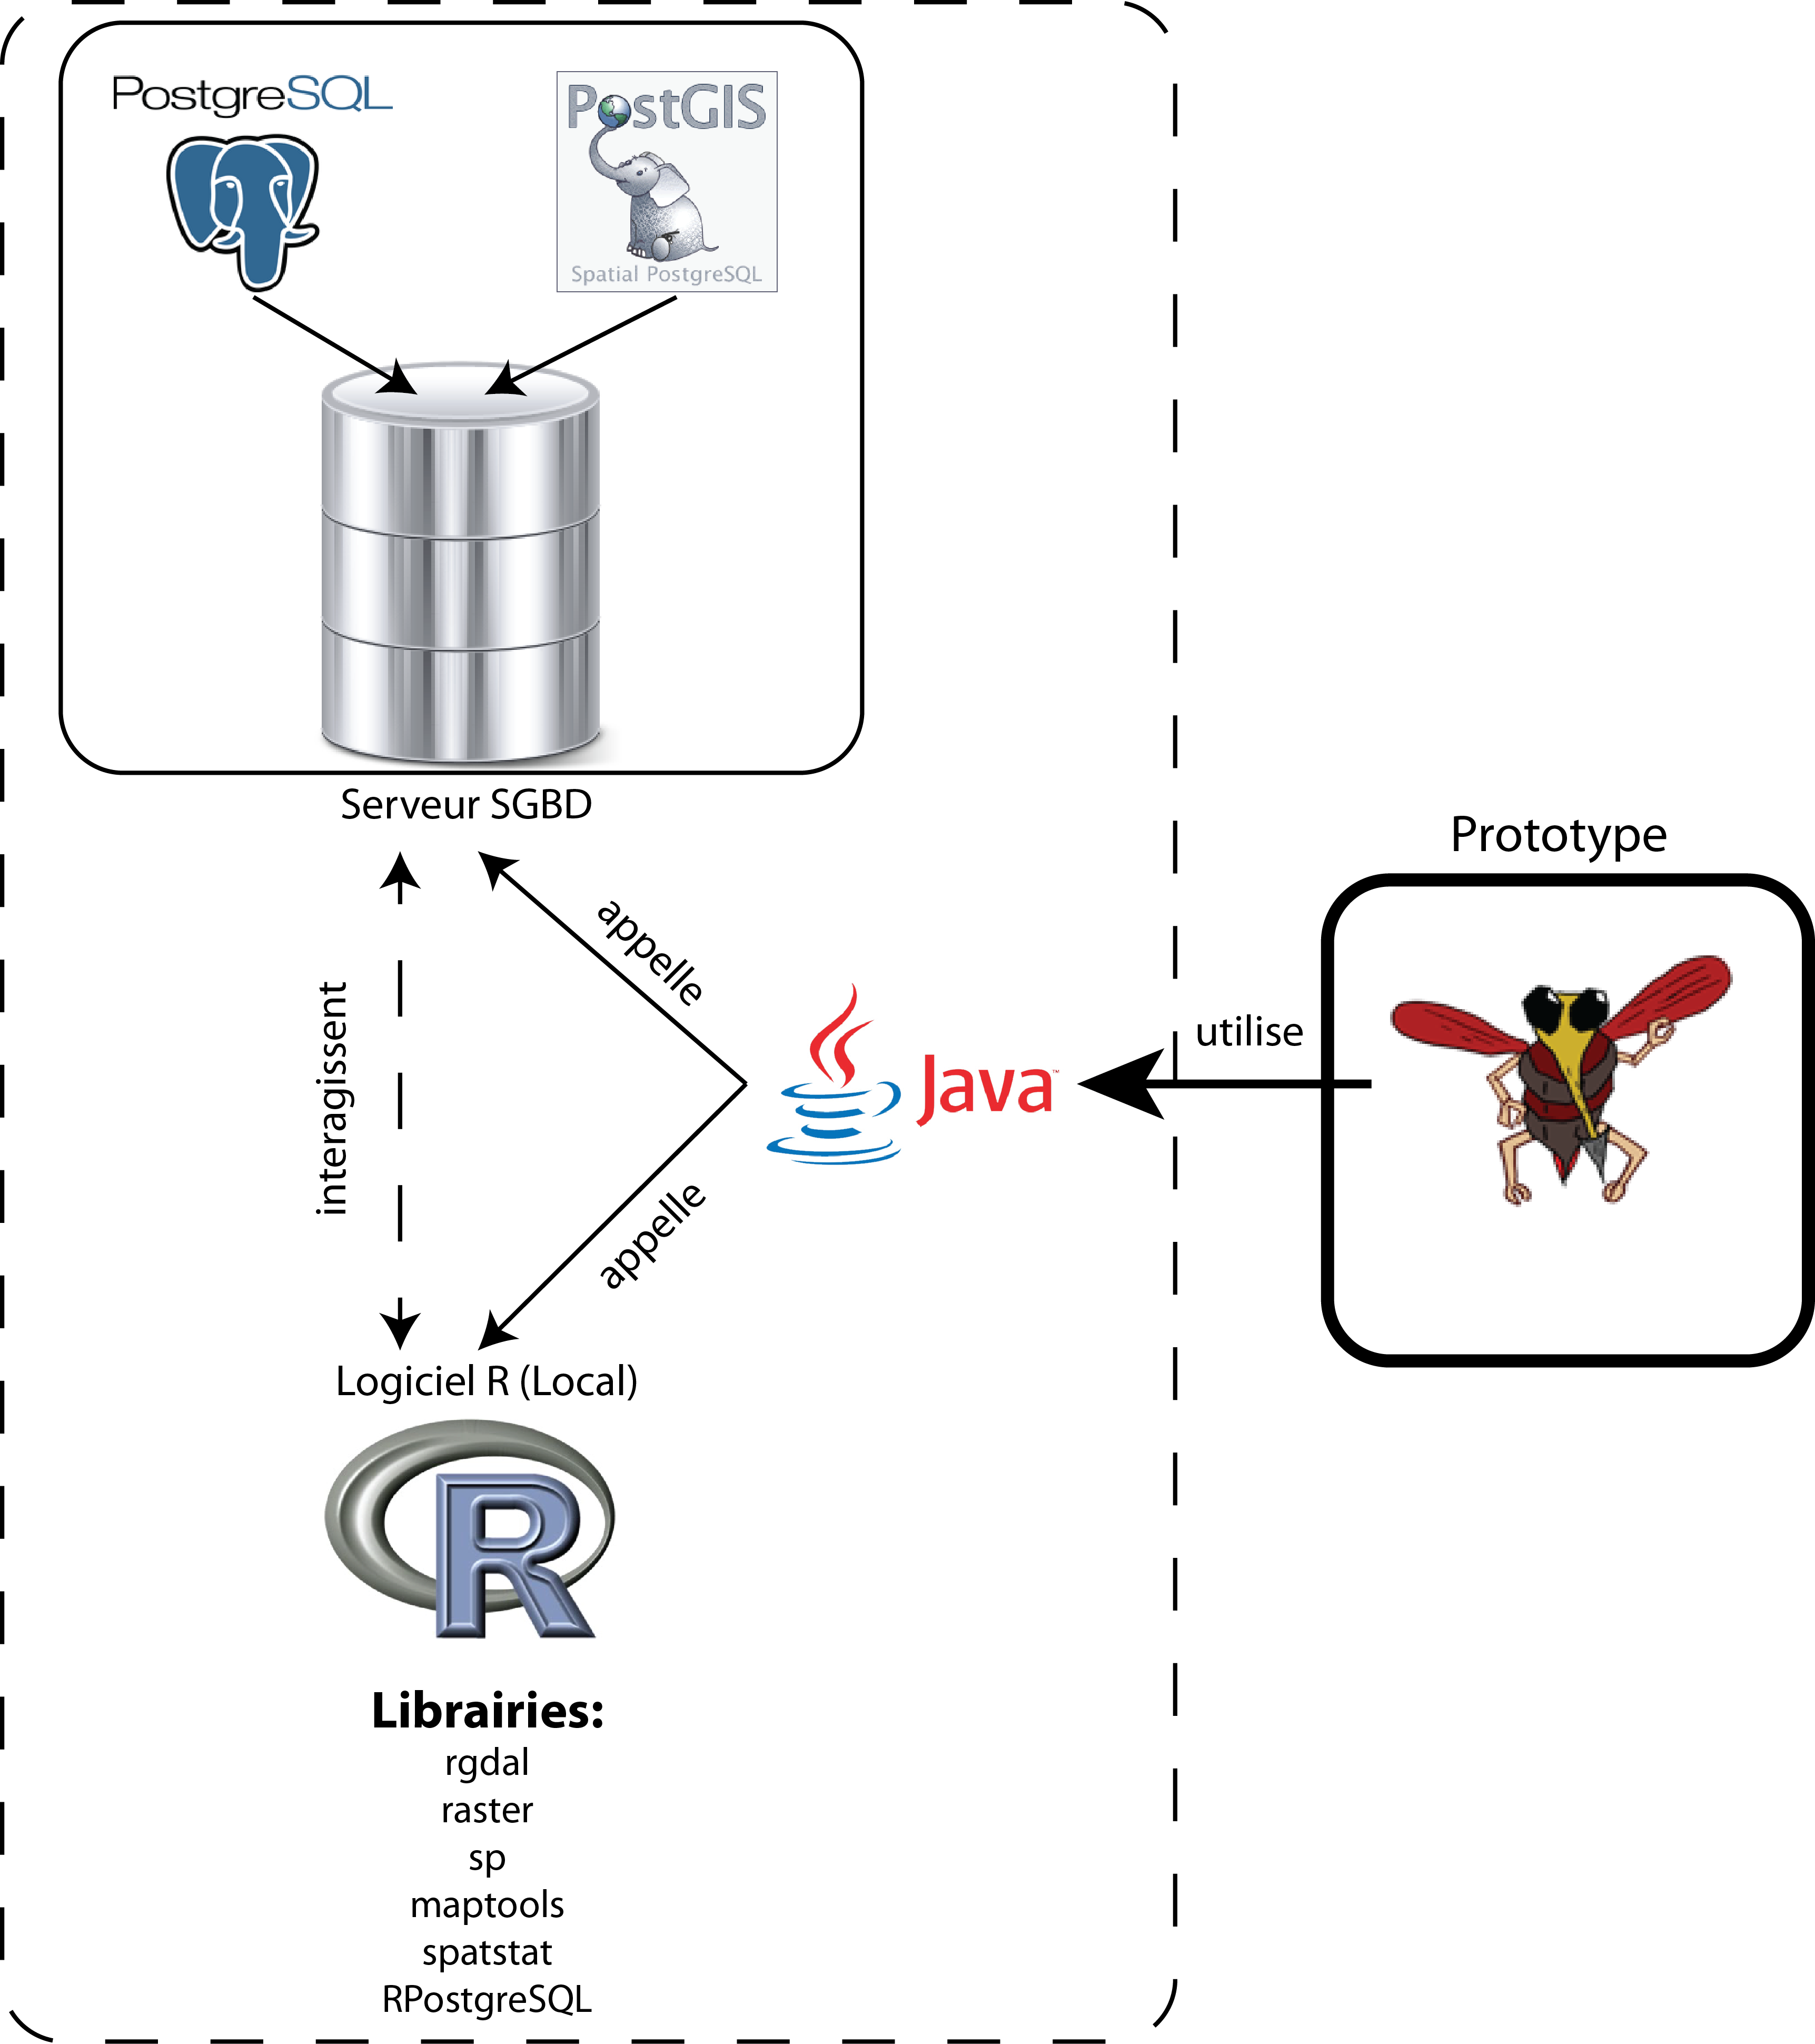
\includegraphics[width=12cm]{Architecture}\\
\caption{\label{Architecture} Architecture informatique du prototype}
\end{center}

\end{figure}


\subsubsection{Présentation de l'outil vision "fermée" (boîte noire)}

Les données utilisées sont insérées dans une base de données \textbf{PostgreSQL} (incluant l'extension \textbf{PostGIS}). Une nouvelle base de données spatiale est créée automatiquement lors de chaque exécution de la chaîne de traitements. Les différentes librairies utiliseront les données dans cette base de données et interagissent entre elles. Par exemple, des données se trouvant dans la base de données \textbf{PostgreSQL} vont être chargées dans \textbf{R} afin de permettre le calcul la densité de population de la zone d'étude.\\

L'architecture informatique est basée exclusivement sur des outils et librairies Open Source et a permis de créer un prototype générique et modulaire. Les fonctions respectivement de PostgreSQL  et de Postgis permettent d'effectuer la majorité des traitements sur des données vecteurs comme des intersections, des buffers ou des unions. Depuis la version 2.0, Postgis gère également les fichiers au format raster. Ainsi, il est désormais possible d'insérer des fichiers raster dans la base de données PostgreSQL ou de transformer des fichiers au format vecteur en format raster. Cette version de Postgis est encore en cours de développement, de nouvelles fonctionnalités raster vont certainement être rajoutées dans le futur. \\

L'outil R permet de manipuler des données aux formats différentes grâce aux nombreuses librairies disponibles pour cet outil. La librairie "spatstat" nous permet par exemple de calculer une densité de population ou d'effectuer une reclassification d'une image raster. La libraire "rgdal" nous permet de disposer des fonctionnalités de la librairie \textbf{GDAL} et de charger dans R les données raster ou vecteurs stockées dans une base de données.\\

Certaines fonctionnalités sont disponibles dans les deux outils et nous avons faits plusieurs tests pour trouver l'outil le plus pertinent par rapport à une problématique. Par exemple la transformation d'un vecteur en raster nécessite beaucoup plus de temps sous R qu'en utilisant la fonction "ST\_Raster" de PostGIS.\\

La multiplicité des fonctions disponibles avec ces deux outils, sachant qu'il existe des librairies R par rapport à de nombreuses problématiques, garantit que cette architecture pourra servir comme base pour un futur développement information du SIEL et être réutilisable par des experts de différents domaines.\\

\subsubsection{Présentation du logiciel vision "ouverte" (boîte blanche)}

Le logiciel ouvert fonctionne sur le même principe que la chaîne de traitements. Le logiciel a été développé en Java et se connecte à un \textbf{SGBD} via un \textbf{JDBC} et au logiciel R via \textbf{RCaller}. En fonction des traitements que l'utilisateur veut effectuer, le logiciel appelle les fonctionnalités PostgreSQL/PostGIS ou R.\\

Néanmoins, un certain nombre de fonctionnalités supplémentaires a été rajouté. Le logiciel est à ce jour un logiciel de création ou de gestion de données, permettant d'insérer, de créer, de modifier ou de supprimer des données dans une base de données spatiale. Ainsi, le logiciel peut intéresser un grande nombre de personnes, spécialistes et non-spécialistes dans le domaine des \textbf{SIG} ou des base de données.\\



\section{Opérationnalisation}

\subsection{Fonctionnement chaine de traitements "fermée"}


\paragraph{Choix des fichiers d'entrée\\\\}

L'utilisateur choisit les données d'entrée. Seules des données au format shape (vecteur) peuvent être sélectionnées. L'utilisateur doit choisir au moins deux fichiers de données : les données correspondant aux bâtiments et les données correspondant aux surfaces aquatiques de la zone d'étude (conformément aux facteurs de risque retenus); et au maximum cinq données (correspondant aux données dont nous disposons).\\

\begin{figure}[H]
\begin{center}
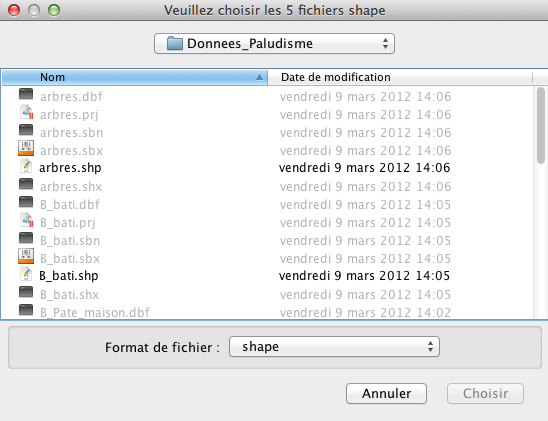
\includegraphics[width=10cm]{Chaine1}\\
\caption{\label{Chaine1} Choix fichiers d'entrée}
\end{center}
\end{figure}


\paragraph{Correspondance des couches\\\\}

Par rapport aux données sélectionnées par l'utilisateur, il est nécessaire de connaître quelle information correspond à quelle donnée. L'utilisateur choisit donc par exemple que la couche "b\_bati" correspond à l'information sur les bâtiments de la zone d'étude et la chaîne gardera en mémoire cette information pour la suite des traitements.\\

\begin{figure}[H]
\begin{center}
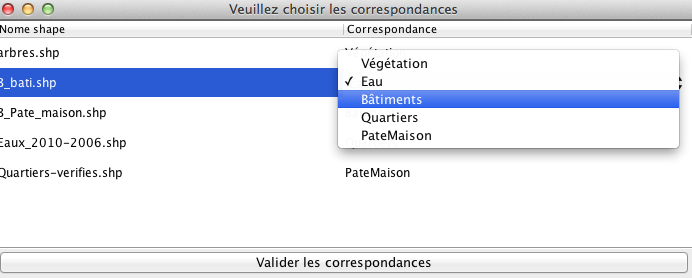
\includegraphics[width=10cm]{Chaine3}\\
\caption{\label{Chaine3} Correspondances des données}
\end{center}
\end{figure}

\paragraph{Création d'une nouvelle base de données spatiale\\\\}

La chaîne de traitements crée une nouvelle base de données. Ceci nécessite un certain nombre d'informations : l'hôte sur lequel PostgreSQL / PostGIS sont installés (localhost si installation en local sur l'ordinateur), le port sur lequel PostgreSQL / PostGIS sont installés, le nom d'utilisateur pour la base de données, le nom de la nouvelle base de données, le mot de passe et la \textbf{projection} souhaités pour la base de données.\\

\begin{figure}[H]
\begin{center}

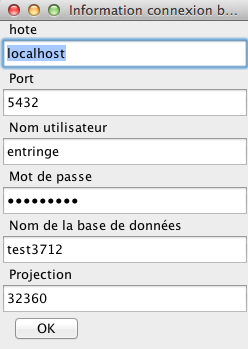
\includegraphics[width=6cm]{Chaine2}\\
\caption{\label{Chaine2} Informations création base de données}
\end{center}

\end{figure}





\paragraph{Insertion des données vectorielles dans la base de données\\\\}

A l'aide du module de transformation shp2pgsql les données vectorielles sont insérées dans la base de données. Ce module transforme les fichiers au format ".shp" en fichiers ".sql" qui sont par la suite insérés dans la base de données à l'aide de la fonctionnalité "pgsql".\\

\begin{figure}[H]
\begin{center}
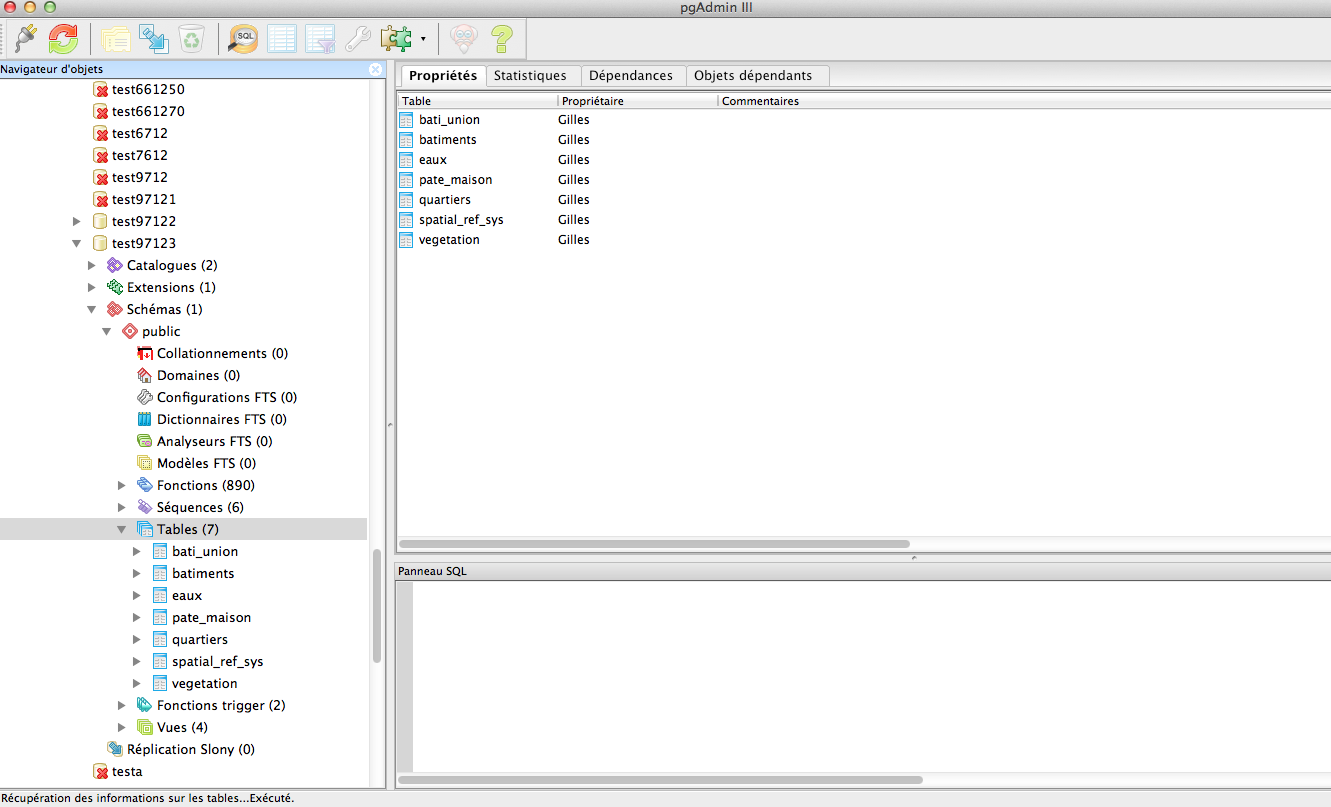
\includegraphics[width=10cm]{Chaine4}\\
\caption{\label{Chaine4} Base de données avec données insérées}
\end{center}
\end{figure}


\paragraph{Nombre d'habitants\\\\}

L'outil demande à l'utilisateur le nombre d'habitants pour la zone d'étude.\\

\begin{figure}[H]
\begin{center}
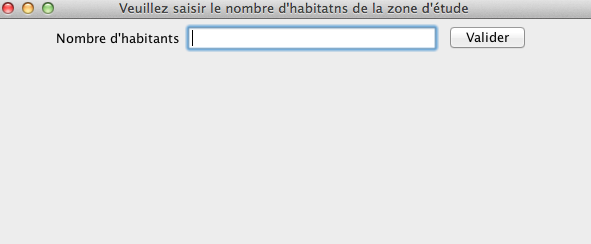
\includegraphics[width=10cm]{Chaine5}\\
\caption{\label{Chaine5} Nombre d'habitants}
\end{center}
\end{figure}


\paragraph{Calcul densité de population et taille pixel\\\\}

L'outil calcule automatiquement, à partir de la couche qui correspond aux bâtiments, la densité de population de la zone d'étude et la taille de cellule qu'un habitant occupe en théorie. Par exemple, pour une population de 15.000 habitants sur une superficie totale de 300.000 mètre carrés, nous effectuons le calcul suivant: \\

300.000/15.000 = 20 m2 par habitants\\
1 habitant = √(20)
1 habitant = 1 cellule = 4.47 * 4.47 m

Un habitant correspond donc en théorie à 20 mètres carrés et à une taille de cellule théoriques de 4.47 * 4.47 mètres.\\


\begin{figure}[H]
\begin{center}
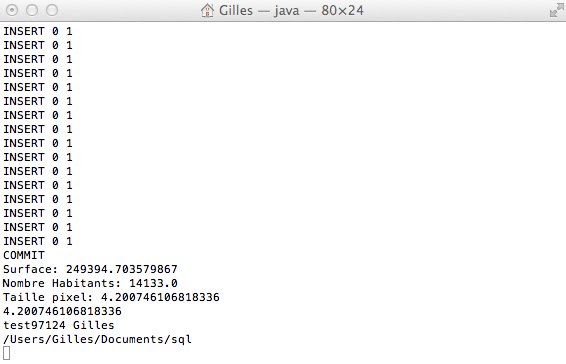
\includegraphics[width=10cm]{Chaine6}\\
\caption{\label{Chaine6} Taille de cellule / Densité de population}
\end{center}
\end{figure}

\paragraph{Calcul et affichage carte de vulnérabilité\\\\}

A partir des différentes opérations et calculs, l'outil calcule une densité des points, affiche et stocke une carte de vulnérabilité.\\

\begin{figure}[H]
\begin{center}
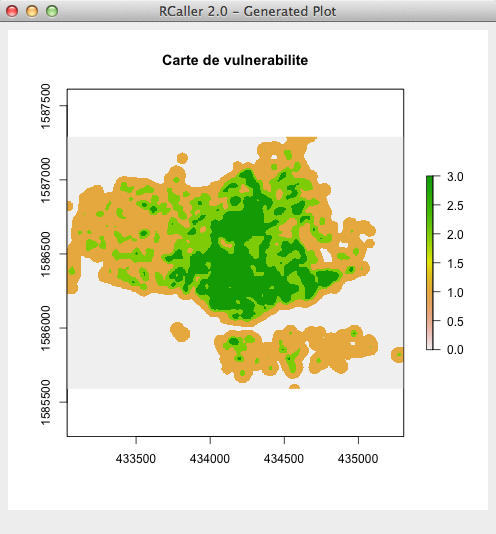
\includegraphics[width=7cm]{Chaine7}\\
\caption{\label{Chaine7}Carte de vulnérabilité}
\end{center}
\end{figure}


\paragraph{Suppression des surfaces aquatiques polluées\\\\}

Par rapport aux données que nous possédons, il est nécessaire de supprimer des surfaces aquatiques polluées car les moustiques ne peuvent pas survivre dans les eaux polluées. L'outil permet de sélectionner quelles surfaces sont polluées à partir d'une colonne de la \textbf{table} de la base de données qui permet à l'utilisateur d'identifier ces surfaces. \\


\begin{figure}[H]
\begin{center}
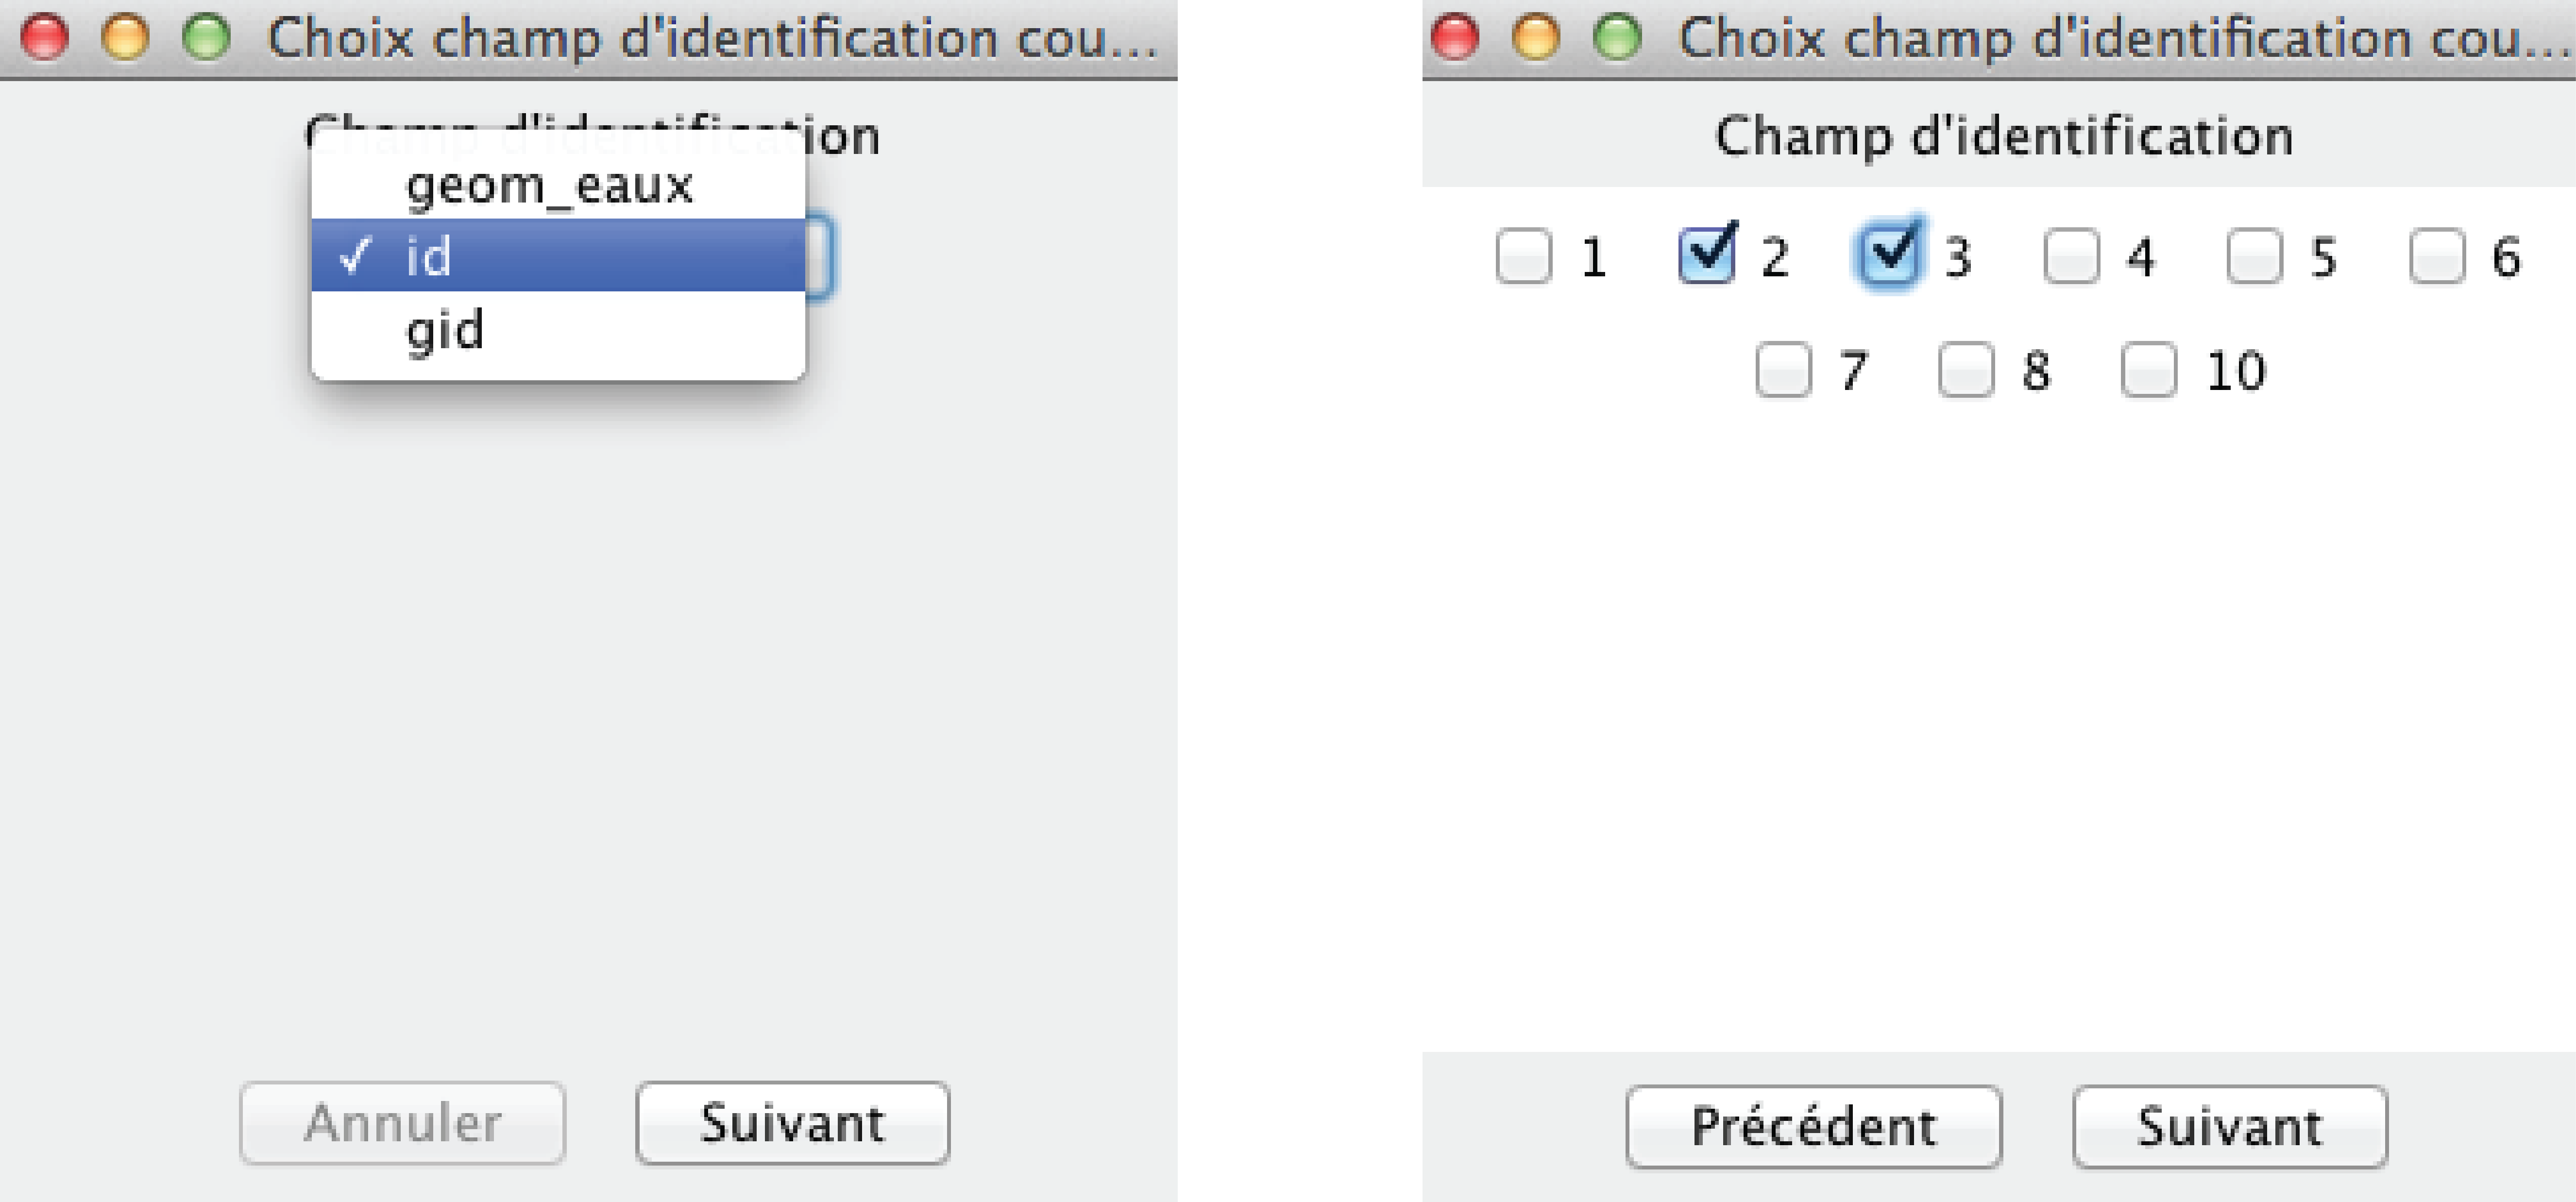
\includegraphics[width=13cm]{Chaine13}\\
\caption{\label{Chaine13}Supprimer surfaces aquatiques polluées}
\end{center}
\end{figure}



\paragraph{Carte d'aléa\\\\}

La carte d'aléa est calculée en combinant plusieurs opérations et traitements d'analyse spatiale : Intersection, création de \textbf{zones tampon}, Union, extent (emprise géographique). Comme il n'y aura pas de risque dans les zones où il n'y pas de vulnérabilité, il est intéressant de supprimer les parties concernant l'aléa qui n'intersectent pas avec la carte de vulnérabilité. Finalement nous obtenons donc une carte d'aléa. Cette carte, en combinaison avec la carte de vulnérabilité crée une carte de risque de transmission, affichée à la fin du traitement.

\begin{figure}[H]
\begin{center}
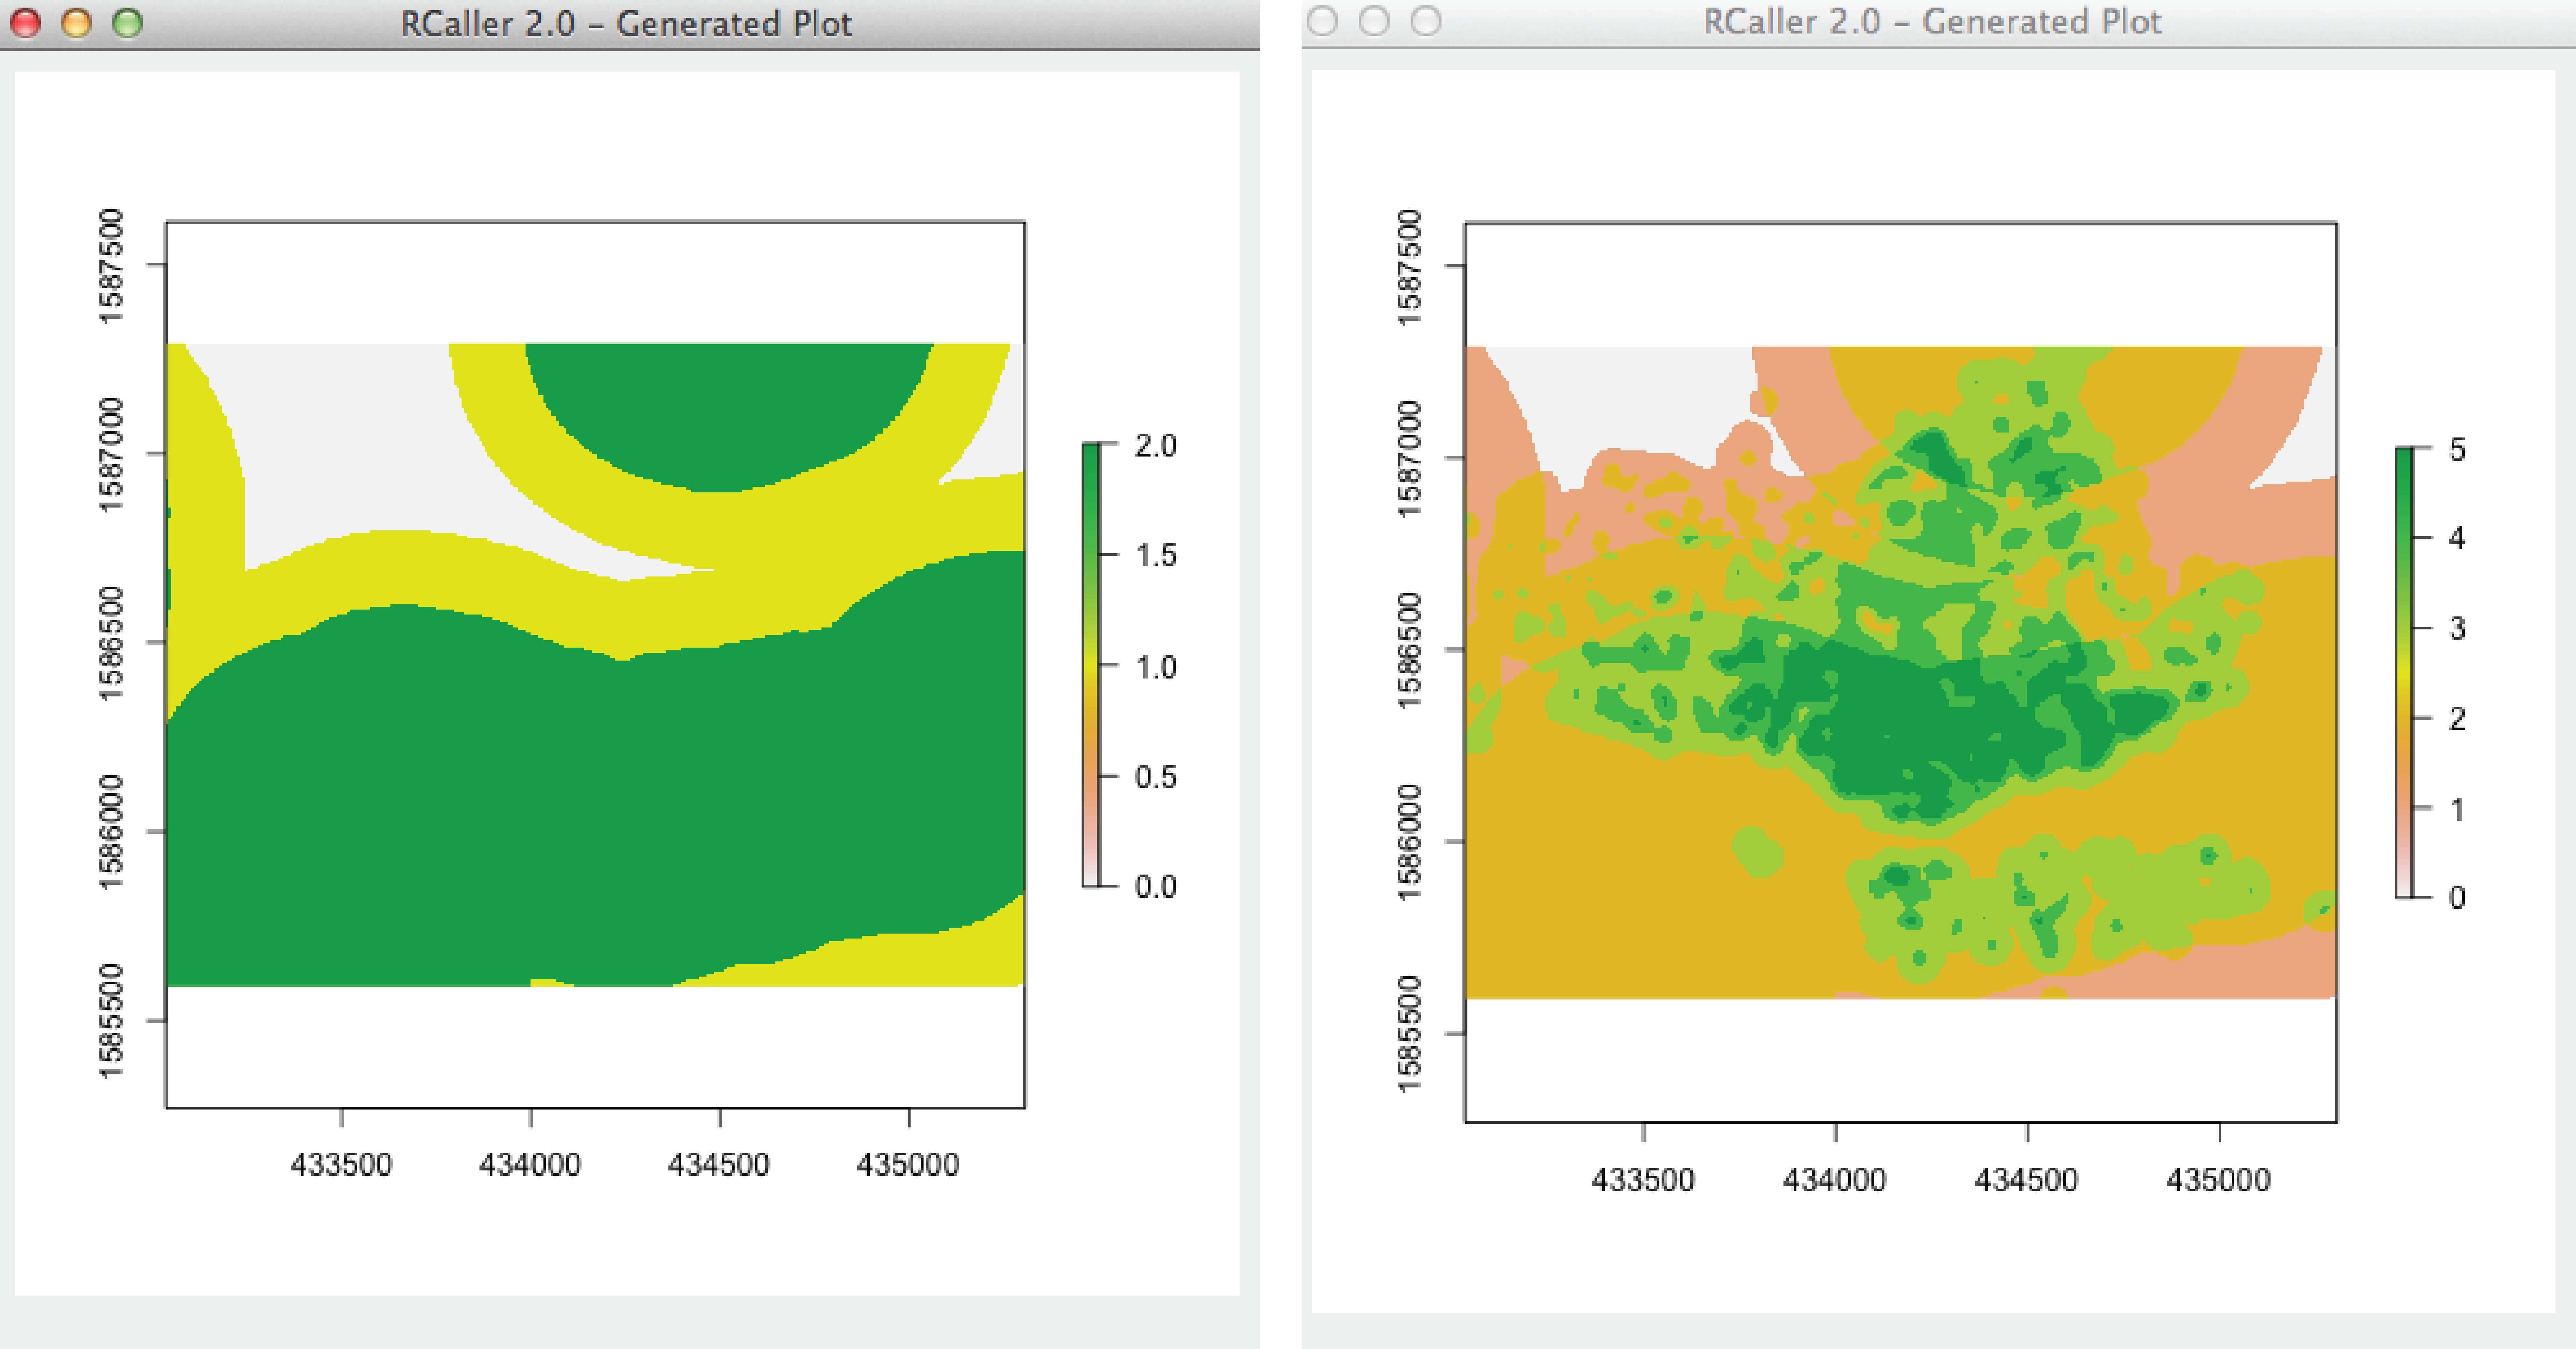
\includegraphics[width=13cm]{Chaine12}\\
\caption{\label{Chaine12}Exemple de carte d'aléa et carte de risque}

\end{center}
\end{figure}

\newpage

%%\subsection{Architecture informatique du logiciel ouvert}

\subsection{Fonctionnement du logiciel "ouvert"}

Le l\textbf{ogiciel ouvert} utilise les mêmes librairies et bibliothèques (R, PostGis, PostgreSQL) que la chaîne de traitements fermée. Au fur et à mesure de l'avancement du développement du logiciel, nous avons rajouté certaines fonctionnalités que nous avons jugées importantes pour l'utilisation du logiciel, comme par exemple l'export des données ou la possibilité de renommer les tables de la base de données. Dans cette partie sera illustrée l'implémentation de l'outil à partir des fonctionnalités les plus intéressantes et innovantes.

\paragraph{Choix emplacement des données\\\\}

L'utilisateur dispose de trois choix possibles par rapport à l'emplacement des données qu'il souhaite traiter :

\begin{itemize}

\item Données dans une base de données PostGIS existante : les données stockées dans la base sont utilisées 
\item Données sur disque dur : une nouvelle base de données est créée
\item Données sur disque dur et dans base de données : des données sont insérées dans une base de données existantes
\end{itemize}


\begin{figure}[H]
\begin{center}
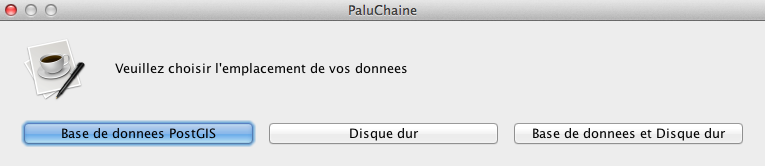
\includegraphics[width=10cm]{Logiciel1}\\
\caption{\label{Traitement1}Choix de l'emplacement des données}

\end{center}
\end{figure}

\paragraph{Information connexion base de données\\\\}

L'utilisateur indique les informations relatives à la base de données. En fonction du choix précédent (emplacement des données), les données stockées dans une base de données existante sont chargées ou une nouvelle base de données est créée et les données des fichiers sélectionnées par l'utilisateur y sont stockées. De plus, l'utilisateur indique la projection de la base de données. Lors de la création d'une nouvelle base de données, toutes les données sont projetées par rapport à cette information, dans le cas d'une base de données existante, toutes les données stockées dans la base sont analysées et, si nécessaire, reprojetées.

\begin{figure}[H]
\begin{center}
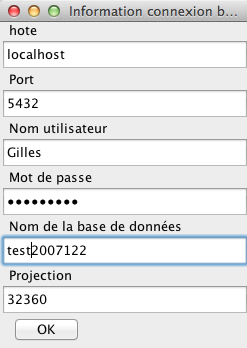
\includegraphics[width=4cm]{Logiciel2}\\
\caption{\label{Traitement2}Informations base de données}
\end{center}
\end{figure}

\paragraph{Menu du logiciel\\\\}

Un menu présente les différents traitements en fonction des catégories de traitements définies  auparavant (cf. \ref{catdonnees}). L'utilisateur peut choisir indépendamment les traitements qu'il souhaite effectuer. 

\begin{figure}[H]
\begin{center}
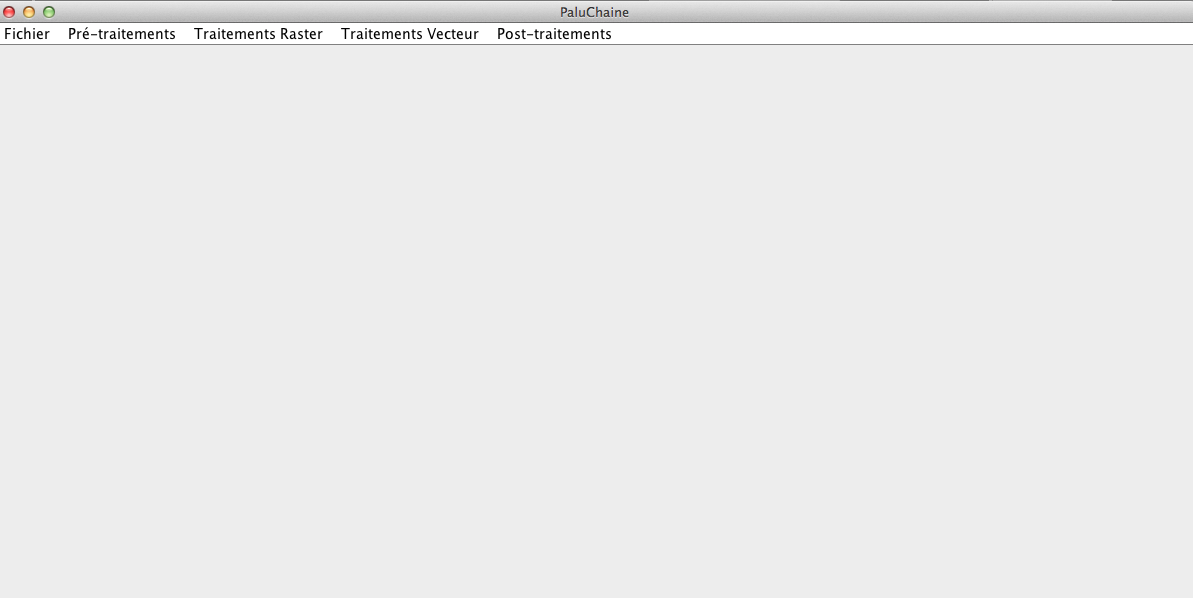
\includegraphics[width=12cm]{Logiciel3}\\
\caption{\label{Traitement2}Le menu de l'outil}
\end{center}
\end{figure}


\paragraph{Les traitements possibles\\\\}

En fonction des catégories de traitements définies auparavant, les traitements suivants peuvent être effectués :

\textbf{Pré-traitements:}\\

\begin{itemize}
\item Insertion de données raster et  vecteur dans la base de données
\item Suppression de données  raster et  vecteur stockées dans la base de données\\

\textbf{Traitements:}\\\\
\textit{Analyse Spatiale}
\item Intersection entre des couches vecteurs
\item Union entre des couches vecteurs
\item Création des zones tampons
\item Calcul de la différence entre deux couches vecteur
\item Création d'une couche représentant l'emprise d'une couche\\\\ \textit{Statistique}
\item Calcul de la surface totale d'une couche
\item Calcul de la taille théorique d'une cellule (cf. Chaîne de traitements)
\item Calcul d'une densité des points à partir d'une couche vecteur\\\\
\textit{Transformation}

\item Rastérisation de couches vecteurs
\item Changement de la projection de la base de données\\

\textbf{Post-traitements}\\
\item Suppression de certaine information d'une couche
\item Reclassification un raster
\item Combinaison de plusieurs rasters
\item Renommage des données dans la base (raster et vecteur)
\item Visualisation de données vecteur et  raster
\end{itemize}


\paragraph{Spécificités techniques du logiciel}

\subparagraph{Mémoire\\\\}

Le logiciel mémorise les traitements déjà effectués (et ce à des fins de contrôle). Par exemple, il n'est pas possible de calculer une taille théorique d'une cellule sans calculer la surface totale de la donnée auparavant. Lorsque l'utilisateur a calculé la taille de cellule et  veut rastériser une donnée au format vecteur, le logiciel se rappelle du calcul de la cellule effectué auparavant. L'utilisateur peut bien évidemment également saisir manuellement la taille de pixel qu'il souhaite appliquer pour le traitement. \\

Après avoir calculé la superficie pour une donnée, elle n'apparaît plus dans la liste des données disponibles pour effectuer ce traitement. Il en est de même pour le calcul de la taille de pixel.

\subparagraph{Affichage\\\\}

L'utilisateur peut afficher à tout moment les données stockées dans la base de données. Cet affichage se fait sous la forme de la fonctionnalité "plot" du logiciel R. 

\subparagraph{Exporter des données\\\\}

Les données stockées dans la base de données peuvent être exportées. Exemple : L'utilisateur, après avoir créé des zones tampons, peut exporter cette nouvelle donnée (au format shape) et l'utiliser dans le SIG de son choix.

\subparagraph{Gestion des données\\\\}

A tout moment, des nouvelles données (vecteur ou raster) peuvent être insérées dans la base de données. Il est également possible de supprimer des données et de renommer les données (tables).

\paragraph{Aperçus du logiciel ouvert\\\\}

La figure \ref{aperculogiciel} donne un bref aperçu du logiciel et de ses fonctionnalités. 
 
\newpage



\begin{figure}[H]
\begin{center}
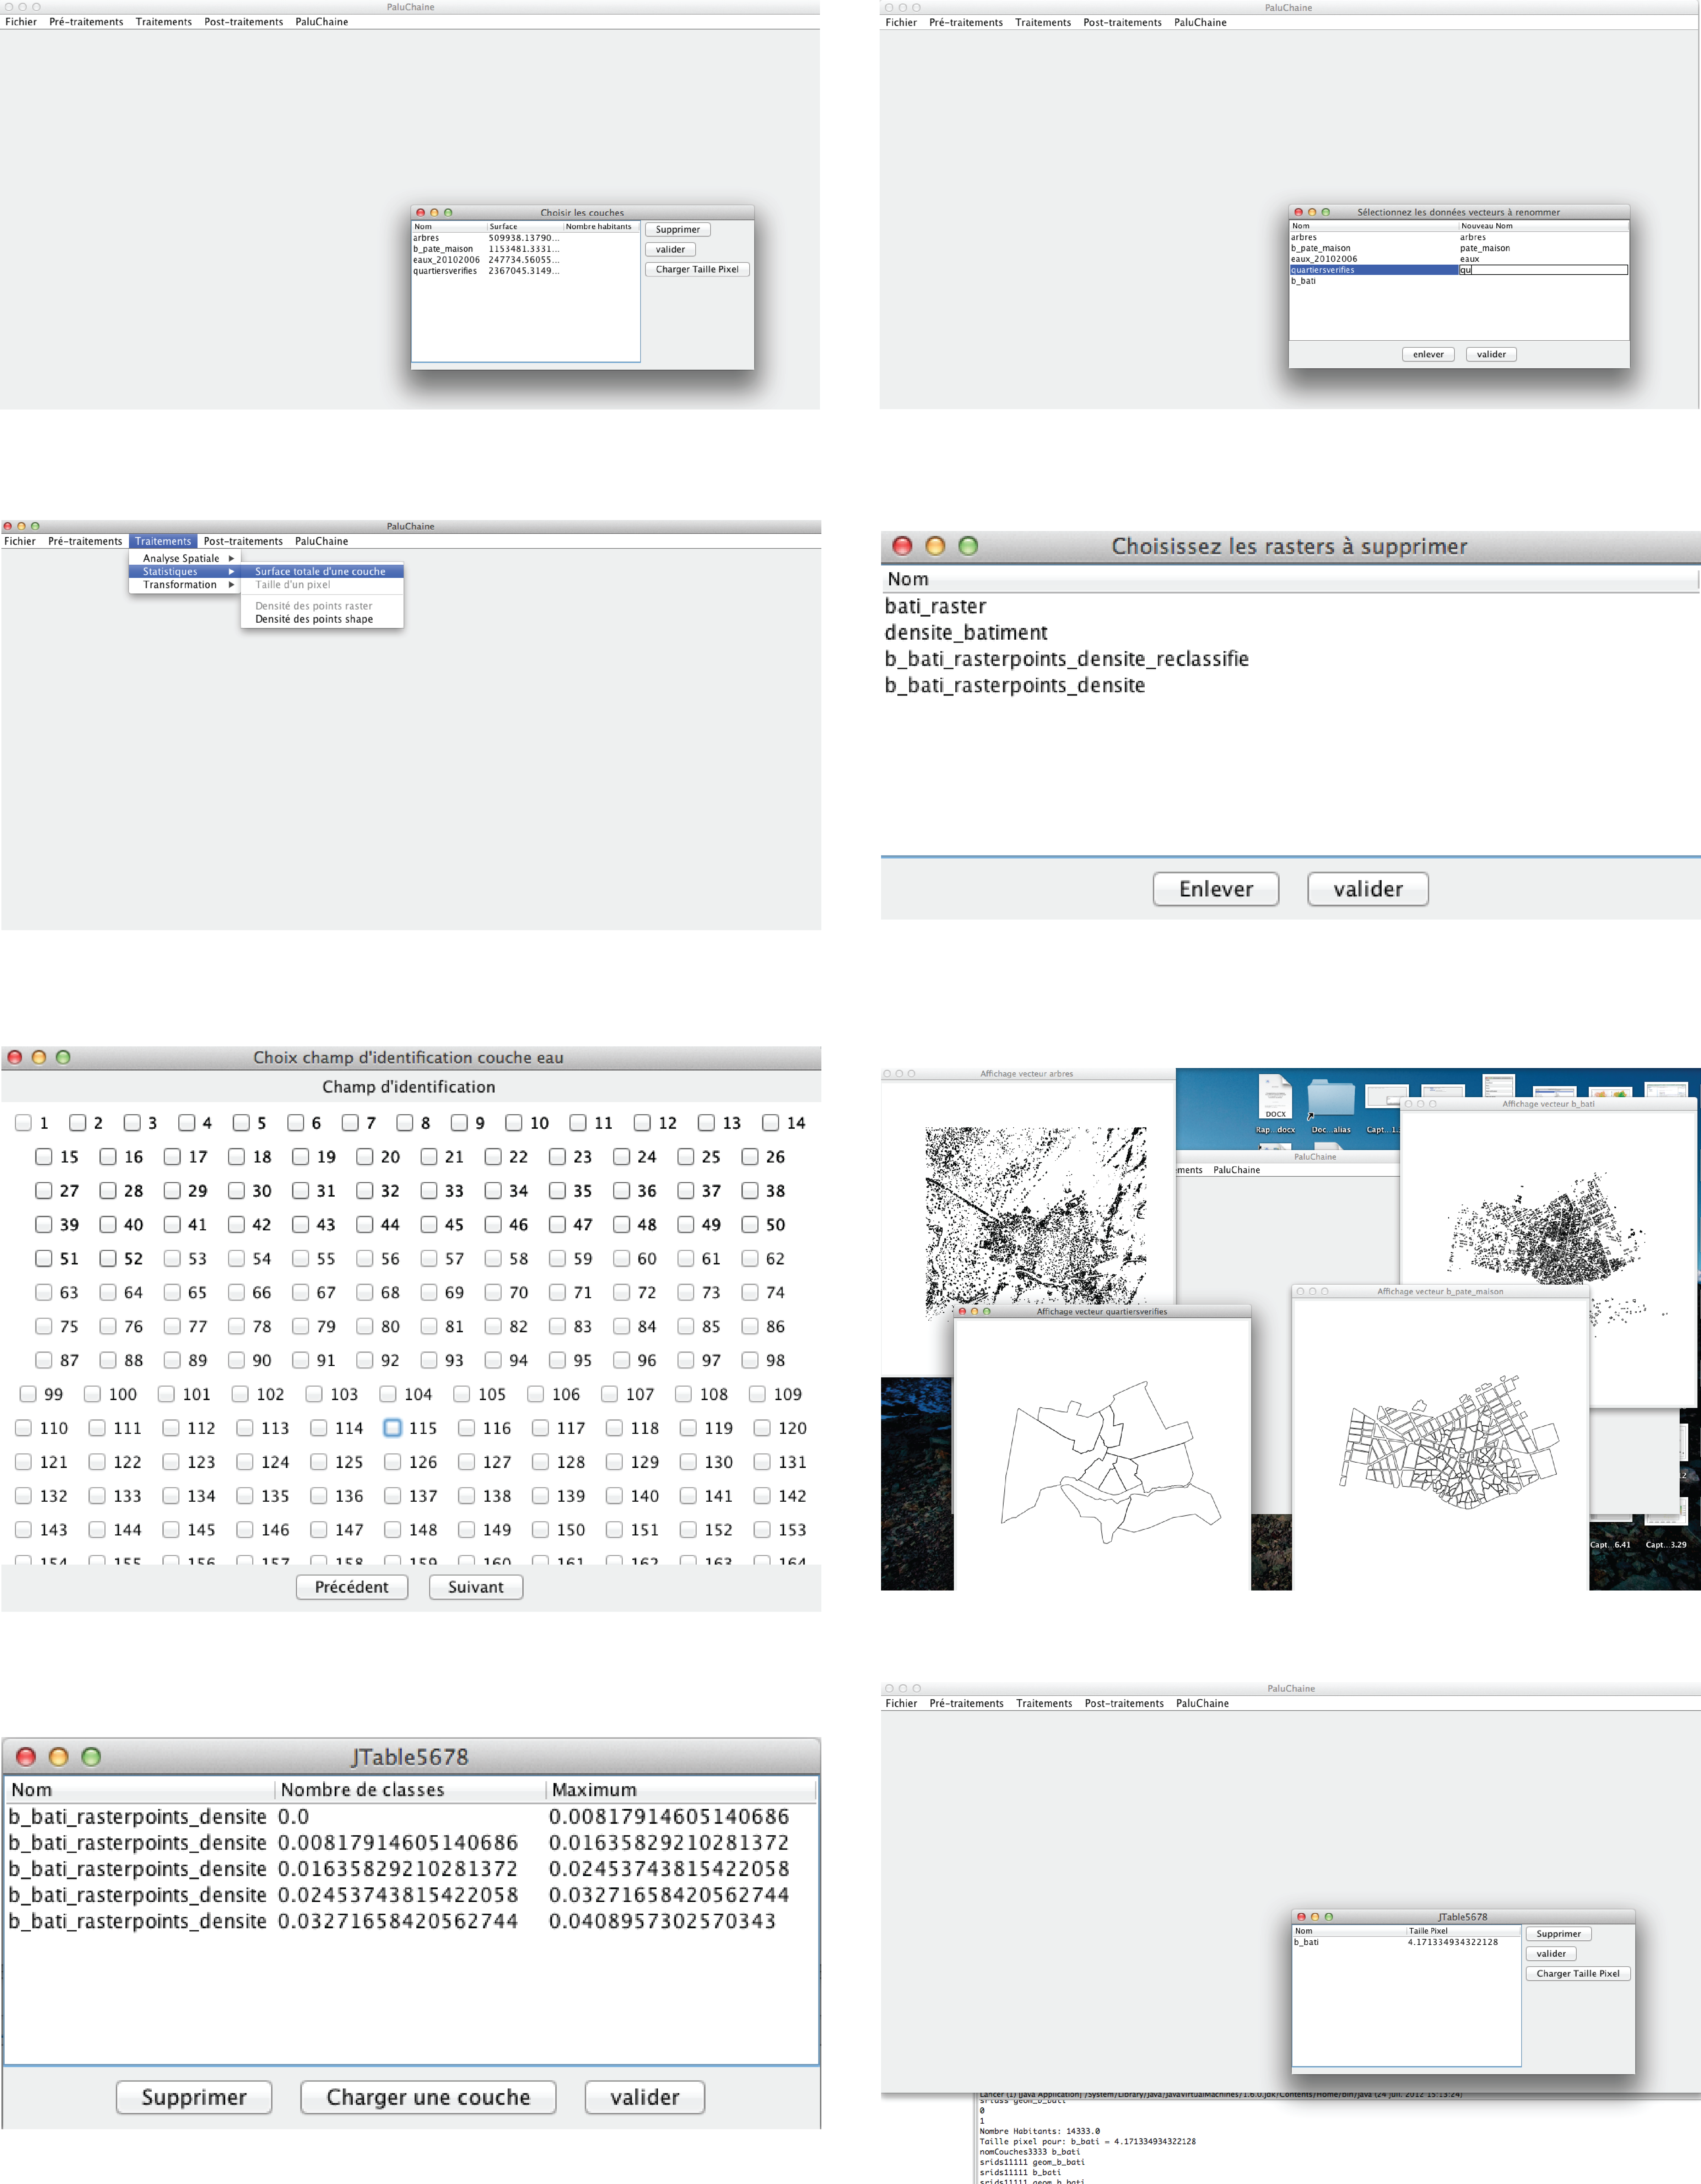
\includegraphics[width=17cm]{Logiciel}\\
\caption{\label{aperculogiciel}Aperçus du logiciel libre}
\end{center}
\end{figure}






